%!TEX root = 00_arbeit.tex

%---------------------------------------------------------------------------------
%% Theorie

\section{Neuronale Netze}
In diesem Kapitel werden zunächst biologische und künstliche neuronale Netze verglichen. Gefolgt von einer Motivation über die Verwendung künstlicher neuronaler Netze (zukünftig als NN bezeichnet) und der Einordnung der NN in die aktuelle Forschungslanschaft. Als nächstes werden die Charakterisierungskriterien für NN vorgestellt und ein Überblick über mögliche Anwendungsgebiete für NN gegeben. Anschließend wird ein Überblick über die Funktionsweise gängiger Modelle gegeben und die Netzwerkmodelle gegenübergestellt.


\subsection{Biologische Neuronale Netze}

Unser Gehirn besteht aus einer Menge an kleinen sowie großen anatomischen Strukturen und kann vereinfachend in vier Bereiche unterteilt werden (siehe \autoref{fig:Gehirn}). Das Großhirn (Telencephalon) ist hierbei für abstrakte Denkaufgaben zuständig. Unterhalb des Großhirns liegt das Kleinhirn (Cerebellum) welches die Motorik koordiniert und steuert. Daneben gibt es noch das Zwischenhirn (Diencephalon) das für die grundlegenden Körpervorgänge zuständig ist. Schließlich verbindet das Stammhirn (Truncus cerebri) das Gehirn mit dem Rückenmark und steuert die Körperreflexe.

\begin{figure}[!htb]
    \centering
        \includegraphics[width=0.5\textwidth]{Bilder/misc/Gehirn.png}
    \caption{Querschnitt des menschlichen Gehirns mit den im Text genannten Arealen.\protect\footnotemark{}}
    \label{fig:Gehirn}
\end{figure}
\addtocounter{footnote}{-1}     % -1 mal die Gesamtanzahl an Fußnoten in der wrapfigure
\addtocounter{Hfootnote}{-1}    % -1 times total number of footnote(mark)s in the wrapfigure
\wrapfigfoot\footnotetext{\autoref{fig:Gehirn} wurde aus \citet[17]{dkriesel07} übernommen.}

In all diesen Bereichen werden Informationen verarbeitet. Dies wird durch Milliarden sehr ähnlicher Zellen bewerkstelligt, welche miteinander kommunizieren. Diese Zellen werden als Neuronen bezeichnet. Der Aufbau und die Verbindung zweier Neuronen ist in \autoref{fig:Neuronen} dargestellt. Betrachtet wird nun der Weg, den die elektrischen Signale in einem Neuron nehmen.

\begin{figure}[!htb]
    \centering
        \includegraphics[width=0.8\textwidth]{Bilder/misc/Neuronen.png}
    \caption{Verbindung zweier Neuronen in einem biologischen neuronalen Netz.\protect\footnotemark{}}
    \label{fig:Neuronen}
\end{figure}
\addtocounter{footnote}{-1}     % -1 mal die Gesamtanzahl an Fußnoten in der wrapfigure
\addtocounter{Hfootnote}{-1}    % -1 times total number of footnote(mark)s in the wrapfigure
\wrapfigfoot\footnotetext{\autoref{fig:Neuronen} wurde aus \citet[2]{sen_an} übersetzt und angepasst.}

Informationen die von anderen Neuronen oder direkt von Sensorzellen kommen werden einem Neuron über die Synapsen übertragen. Die Synapsen liegen meistens auf den Dendriten, welche sich Baumartig vom Soma (dem Zellkern des Neurons) ausbreiten und für die Aufnahme der elektrischen Signale verschiedener Quellen zuständig sind. Die so im Soma eintreffenden Signale wirken entweder anregend oder abschwächend. Das Soma kumuliert die eintreffenden Signale auf und ab einem bestimmten Wert (der als Schwellwert bezeichnet wird) schickt das Soma über das Axon seinerseits einen elektrischen Impuls. Das Axon leitet den Impuls wiederum über Synapsen an die Dendriten eines nachfolgenden Neurons. Abstrakt kann ein Neuron nun als Schalter mit einem Informationsein- und ausgang betrachtet werden.\,\citef[15 ff]{dkriesel07} Die Verbindungen aus mehreren Neuronen werden als neuronales Netz bezeichnet und so bilden verschiedene neuronale Netze unser Gehirn.

\todo{Da fehlt noch etwas Text.}

\subsection{Künstliche Neuronale Netze}\label{sec:einf_neuro}



%\subsection{Globaler Überblick über Neuronale Netze}
%\farbig{[Erklärung der neuronalen Netze... vielfältige Anwendungsgebiete... Hier erforderlich Netze zur Zeitreihenvorhersage]}
%\setlength{\intextsep}{0pt}%

%\begin{wrapfigure}{r}{0.5\textwidth}
%    \centering
%        \includegraphics[width=0.5\textwidth]{Bilder/BNN_ANN.png}
%    \caption{Gegenüberstellung eines Ausschnittes aus einem biologischen neuronalen Netz a)\protect\footnotemark{} und einem künstlichen neuronalen Netz b).}
%    \label{fig:BNN_ANN}
%\end{wrapfigure}


%\citet[\pno~2~ff.]{sen_an}

Künstliche neuronale Netze sind augenblicklich eine Disziplin der Computerbasierten Intelligenz (engl.: computional intelligence)~(CI), welches wiederum einen Teilbereich der Künstlichenintelligenz (engl.: artificial intelligence)~(AI) darstellt. Die CI fasst verschiedene von der Natur inspirierte Berechnungsmethoden zusammen. Neben den NN sind weitere Methoden der CI Fuzzy-Systeme~(FS), Evolutionäre Algorithmen~(EA), Schwarmintelligenz~(SI) und Künstliche Immunsysteme~(AIS).\citef[11 ff]{Kroll16} Obwohl sich diese Arbeit wesentlich mit NN beschäftigen wird, wird an dieser Stelle auf weitere CI-Methoden hingewiesen, da in der Literatur hybride CI-Systeme bekannt sind und auch genutzt werden.

Ein künstliches neuronales Netz (engl. artificial neural networks)~(NN) ist ein mathematisches Konstrukt. Es bildet ein informationsverarbeitendes System welches aus einer Vielzahl einfacher Einheiten den sogenannten Neuronen besteht. Entstanden ist es Anfang der 40er Jahre des letzten Jahrhunderts\citef[A1.1:1]{Fiesler96} aus der Untersuchung von biologischen Abläufen im Nervensystem von Wirbeltieren, wo Sinneseindrücke des Körpers aufgenommen und mit Hilfe diverser neuronaler Netze verarbeitet werden.

\begin{figure}[!htb]
    \centering
        \includegraphics[width=1\textwidth]{Bilder/misc/BNN_ANN.png}
    \caption{Gegenüberstellung eines Ausschnittes aus einem biologischen neuronalen Netz a)\protect\footnotemark{} und einem künstlichen neuronalen Netz b).}
    \label{fig:BNN_ANN}
\end{figure}

\addtocounter{footnote}{-1}     % -1 mal die Gesamtanzahl an Fußnoten in der wrapfigure
\addtocounter{Hfootnote}{-1}    % -1 times total number of footnote(mark)s in the wrapfigure
\wrapfigfoot\footnotetext{\autoref{fig:BNN_ANN} a) wurde aus \citet[2]{sen_an} übersetzt und angepasst.}

\autoref{fig:BNN_ANN} zeigt eine Gegenüberstellung eines künstlichen und biologischen Neurons. Dieser Vergleich ist auf \citet{kneuron} zurückzuführen. Sie formulierten die Funktion eines Neurons wie folgt:\\ Ankommende Informationen werden von den Dendriten aufegenommen. Daraufhin wird die Aktivität der Dendriten  mit einer bestimmten Gewichtung im Soma summiert und wenn ein bestimmter Schwellwert überschritten ist, wird die Information durch das Axon weitergeleitet. Die Kontaktstellen der Neuronen untereinander bilden die Synapsen. Welche das kontaktierte Neuron erregen oder hemmen können.\citef[17]{bio_neuron} Hirbei können die Dendriten eines biologischen Neurons als Informationseingang, das Axon als Informationsausgang, die Synapsen als Gewichte und die Soma als Propagierungs- und Aktivierungsfunktion des künstlichen Neurons angesehen werden. Die Aufgabe der Propagierungsfunktion ist es die ankommenden Signale zu verarbeiten und für die Aktivierrungsfunktion vorzubereiten. Wobei die Aktivierungsfunktion dann entscheidet wie mit den Informationen umgegangen werden soll.

%\todo{Als Grundmodell für das künstliche Neuron diente das neurophysiologische Vorbild, das auf McCulloch und Pitts (aaO.) zurtickzuführen ist. Diese betrachteten ein Neuron als eine Art Addierer der ankommenden Impulse, die durch die Dendriten (Eingangs-kanäle) aufgenommen werden. Die Aktivitaten, mit einer bestimmten Gewichtung, werden im Soma (Korper des Neurons mit Zellkem) summiert und, sofern die Summe einen bestimmten Schwellwert überschreitet, wird die Information durch das Axon (Ausgangskanal) weitergeleitet. Der Kontakt zu den anderen Neuronen findet über Synapsen (elektrochemische Kontakte) statt. Diese können die kontaktierten Neuronen hemmen bzw. erregen (vgl. Stanley und Bak, 1991; Brause, 1991; Schoneburg u.a., 1990; Ritter u.a., 1991)  $doi:https://doi.org/10.1007/978-3-322-83450-8\_2 - S.17$}

Das zurzeit prominenteste künstliche Neuron, dargestellt in \hbox{\autoref{fig:BNN_ANN} b)}, wird nach \citet{perceptron_ros58} als Perceptron bezeichnet. %Es verarbeitet zunächst die Eingangssignale über die Propagierungsfunktion (in \autoref{fig:BNN_ANN} b) ist es die Summenfunktion).
So summiert es zunächst die gewichteten Eingangsinformationen mit der Propagierungsfunktion $\varphi (x)=\sum_{i=1}^{n}x_{i}\omega_{i}$, anschließend wird die gewichtete Summe~$\varphi(x)$ über die Aktivierungsfunktion~$\sigma(x)$ als Ausgang~$y$ an das nächste Neuron übergeben.
%
%
%\setlength{\intextsep}{0pt}%
%\setlength{\columnsep}{10pt}%
%\begin{wraptable}{l}{6.4cm}
%    \caption {Analogie zwischen biologischen und künstlichen Neuronen.}
%   \begin{tabular}{>{\centering\arraybackslash}m{2.2cm}>{\centering\arraybackslash}m{3.4cm}}
%    \hline
%    Biologisches\newline Neuron & Künstliches\newline Neuron            \\ \hline \hline
%    Soma                & Summen- und\newline Aktivierungsfunktion      \\ 
%    Dendrit             & Eingang                                       \\ 
%    Axon                & Ausgang                                       \\ 
%    Synapse             & Gewicht                                       \\ \hline
%    \end{tabular}
%    \label{tab:BNN_ANN}
%\end{wraptable}
%
Klassische Aktivierungsfunktionen sind in \autoref{fig:funktion} dargestellt. Wobei die \hbox{Heaviside-,} die lineare Schwellwertfunktion und der Tangens Hyperbolicus bipolar dargestellt sind (Wertebereich [-1,1]) aber auch unipolar (Wertebereich [0,1]) verwendet werden können. Die logistische Funktion weist zwar nur einen Wertebereich von [0,1] auf aber durch den Temperaturfaktor kann sie an die Heavisidefunktion angenährt werden und hat den Vorteil der Differenzierbarkeit.\footnote{Vgl. \citet[5]{neuralnet_intro} und \citet[39 f]{dkriesel07}.}
%\ErrorsOff*
\begin{figure}[!htb]
    \centering
    %\WarningsOff*
    
    \includestandalone[mode=image|tex]{Bilder/misc/Aktivierungsfunktionnen}
    %\documentclass[tikz,border=0pt]{standalone}%
\usepackage{tikz-cd}
%\usepackage{silence}
\usetikzlibrary{arrows}
%\ErrorsOff*

\begin{document}
        %---------------------------------------------------------------
        %% Heaviside
        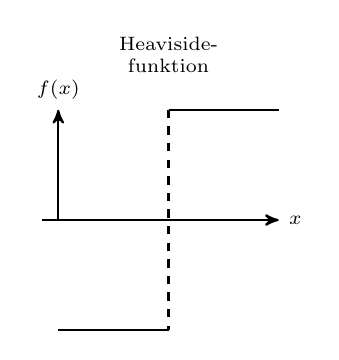
\begin{tikzpicture}[scale=.7,font=\scriptsize,thick,>=stealth']
            \coordinate (O) at (0,0);
            % horizontal axis
            \draw[->] (-0.3,0) -- (4,0) coordinate[label = {right:$x$}] (xmax);
            % vertical axis
            \draw[->] (0,0) -- (0,2) coordinate[label = {above:$f(x)$}] (ymax);
  
            \node[align=center] at (2,3) {Heaviside-\\funktion};
  
            \draw (2,2) -- (4,2);
            \draw (2,-2) -- (0,-2);
            \draw[dashed] (2,2) -- (2,-2);
        \end{tikzpicture}
        %---------------------------------------------------------------
        %% lineare Schwellwertfunktion
        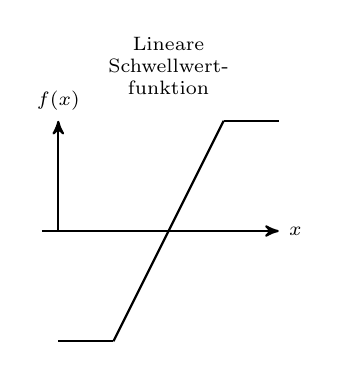
\begin{tikzpicture}[scale=.7,font=\scriptsize,thick,>=stealth']
            \coordinate (O) at (0,0);
            % horizontal axis
            \draw[->] (-0.3,0) -- (4,0) coordinate[label = {right:$x$}] (xmax);
            % vertical axis
            \draw[->] (0,0) -- (0,2) coordinate[label = {above:$f(x)$}] (ymax);
  
            \node[align=center] at (2,3) {Lineare\\Schwellwert-\\funktion};
  
            \draw (3,2) -- (4,2);
            \draw (1,-2) -- (0,-2);
            \draw (1,-2) -- (3,2);
        \end{tikzpicture}
        %---------------------------------------------------------------
        %% Fermifunktion
        \begin{tikzpicture}[scale=.7,font=\scriptsize,thick,>=stealth']
            \draw[white] (1,-2) -- (3,2);
            
            \draw[scale=.5,domain=-4:4,smooth,variable=\x,lightgray]      plot ({\x+4},{4*(1/(exp(-\x/.2)+1))});
            \draw[scale=.5,domain=-4:4,smooth,variable=\x,lightgray]      plot ({\x+4},{4*(1/(exp(-\x/.5)+1))});
            \draw[scale=.5,domain=-4:4,smooth,variable=\x,black]          plot ({\x+4},{4*(1/(exp(-\x/.8)+1))});
            % horizontal axis
            \draw[->] (-0.3,0) -- (4,0) coordinate[label = {right:$x$}] (xmax);
            % vertical axis
            \draw[->] (0,0) -- (0,2) coordinate[label = {above:$f(x)$}] (ymax);
            \node[align=center] at (2,3) {Logistische\\Funktion};
        \end{tikzpicture}
        %---------------------------------------------------------------
        %% Tangens Hyperbolicus
        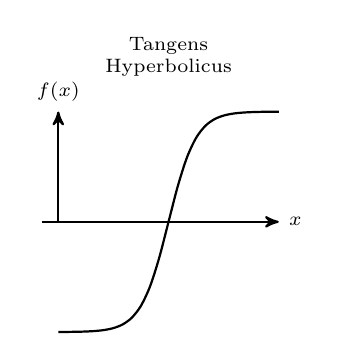
\begin{tikzpicture}[scale=.7,font=\scriptsize,thick,>=stealth']
            \coordinate (O) at (0,0);
            % horizontal axis
            \draw[->] (-0.3,0) -- (4,0) coordinate[label = {right:$x$}] (xmax);
            % vertical axis
            \draw[->] (0,0) -- (0,2) coordinate[label = {above:$f(x)$}] (ymax);
            \node[align=center] at (2,3) {Tangens\\Hyperbolicus};
            \draw[scale=0.5,domain=-4:4,smooth,variable=\x,black] plot ({\x+4},{4*tanh(\x)});
        \end{tikzpicture}
\end{document}
    \caption{Typische Funktionen die als Aktivierungsfunktion angewendet werden.\protect\footnotemark{}}
    \label{fig:funktion}
\end{figure}
\addtocounter{footnote}{-1}     %  -1 mal die Gesamtanzahl an Fußnoten in der wrapfigure
\addtocounter{Hfootnote}{-1}    % -1 times total number of footnote(mark)s in the wrapfigure
\wrapfigfoot\footnotetext{\autoref{fig:funktion} wurde in Anlehnung an \citet[5]{neuralnet_intro} Figure 1.5 erstellt.}

%\,\autoref{fig:SOM_top} wurde aus \citet[274]{Kroll16} übernommen.


%\newpage



\subsection{Charakterisierung und Anwendung künstlicher neuronaler Netze}

Da es nicht das NN gibt sondern viele unterschiedliche Arten, die teilweise spezielle Anwendungsgebiete finden, werden in diesem Unterkapitel Charakterisierungskriterien für NN vorgestellt. Schließlich wird ein Überblick über mögliche Anwendungsgebiete gegeben.\\

\begin{figure}[!htb]
    \centering
        \includegraphics[page=1,width=1\textwidth,trim={.5cm 6cm 0 .6cm},clip]{Bilder/misc/ANN_Organigramme.pdf}
    \caption{Organigramm der Kriterien zur Charakterisierung künstlicher neuronaler Netze.}
    \label{fig:ann_charakterisierung}
\end{figure}


Im allgemeinen können NN anhand der in \autoref{fig:ann_charakterisierung} dargestellten Kategorien charakterisiert werden\citef[7 ff]{characterisation_4}:%

\begin{enumerate}
\item%
Nach der Art des verwendeten Neurons.\\
Dazu gibt es in der Literatur vielfältige Beispiele. \citet{Fiesler96} zählen einige Beispiele im Kapitel B1 auf und weisen auf Unterschiede hin. Als Beispiel wird dort das bereits erwähnte Perceptron beschrieben. Dann gehen sie auf das Neuron des Hopfield-Netzwerkes ein, bei dem das Neuron ein Teilchen beschreibt welches sich in einem Magnetfeld ausrichtet. Ein eher exotischer Vertreter der dort nicht erwähnt wird ist das Fuzzy-Neuron von \citet{fuzzy-neuron}, welches nach der Aktivierung mehrere mögliche Zustände einnehmen kann und seine Anwendung in der Mustererkennug findet.

\item%
Nach der Topologie bzw. der Verbindungsarchitektur.\\
Sie beschreibt wie Neuronen in einem Netzwerk verbunden sind.
Es werden folgende Architekturen unterschieden:
\begin{itemize}
\item[\textbf{$\bullet$}]%
Autoassoziative: Hierbei fungieren die Eingangs- gleichzeitig als Ausgangsneurone (z.B. das Hopfield-Netzwerk). 

\item[\textbf{$\bullet$}]%
Heteroassoziative: Unterschiedliche Neurone übernehmen die Rolle der Eingangs- bzw. Ausgangsneurone. Hierzu zählen die Multi-layer-Perceptrons (MLP) bei dem mehrere Schichten von mehrzahligen Perceptrons ein Netzwerk Bilden\citef[86 ff]{dkriesel07}. Aber auch das Kohonen Netzwerk auch bekannt als Self Organizing Maps (SOM) bei dem die Neuronen sich selbständig anordnen und der Zustand des Netzes als Ausgabe dient\citef[153 ff]{dkriesel07}.

Zusätzlich wird unterschieden wie die Verbindungen unter den einzelnen Neuronen realisiert sind. Hier wird zwischen zwei Arten unterschieden:

\item[$\circ$]%
Feed-Forward: Diese Netzwerke bestehen meistens aus Schichten und eine Schicht ist nur mit der jeweils nächsten Schicht verbunden, sodass die Informationen von Schicht zu Schicht weiter gegeben werden.

\item[$\circ$]%
Recurrent (Feed-Back): In der deutschsprachigen Literatur als rückgekoppelte oder rekurrente Netze bezeichnet beeinflussen sich die Schichten dieser Netzwerke gegenseitig. Die Neuronen dieser Netzwerke besitzen eine Verbindung entweder zu sich selbst (direkte Rückkoppelung), zu den Neuronen der vorhergehenden Schicht (indirekte Rückkopplung), zu den Neuronen der gleichen Schicht (laterale Rückkopplung) oder vollverknüpfte Netze (Verbindungen zwischen allen Neuronen ausgenommen der direkten Rückkopplung). Durch die Rückkopplung besitzen diese Netzwerke ein \glqq Gedächtnis\grqq~da der vorherige Zustand in die Auswertung der aktuellen Eingangsinformation mit einfließt.\citef[42 ff]{dkriesel07} Ein Beispiel für ein vollständig verbundenes Netzwerk ist das Hopfield-Netzwerk.

\end{itemize}

\item%
Nach dem Lernalgorithmus. Dieser ermöglicht es das Netzwerk zu trainieren. Die heutzutage benutzten Algorithmen werden in drei Gruppen unterteilt\footnote{Vgl. \citet[55]{dkriesel07}.\label{kriesel55}}:

\begin{itemize}
\item[\textbf{$\bullet$}]%
Supervised learning (überwachtes Lernen): Die Trainingsbeispiele bestehen aus einer Menge an Eingangsinformationen und den dazugehörigen Ausbangsinformationen. Das Ziel ist es die Differenz zwischen der tatsächlichen Ausgabe des Netzwerks und den vorliegenden Ausgangsinformationen zu minimieren.

\item[\textbf{$\bullet$}]%
Reinforcement learning (bestärkendes Lernen): Plakativ kann diese Lernmethode als Zuckerbrot und Peitsche bezeichnet werden bzw. lernen durch Belohnung und Bestrafung. Hierbei werden die Eingangsinformationen zur Verfügung gestellt und die Ausgabe des Netzwerkes wird anhand einer Belohnungsfunktion bewertet. Wird die Ausgabe als gut/schlecht angesehen so werden die zugehörigen Verbindungen gestärkt/geschwächt\footnote{Vgl. \citet[201]{dkriesel07} und \citet[A2.3:5]{Fiesler96}.}. 

\item[\textbf{$\bullet$}]%
Unsupervised learning (unüberwachtes Lernen): Wird auch als selbstorganisiertes (self organized) Lernen bezeichnet. Die Trainingsbeispiele bestehen hierbei nur aus Eingansinformationen. Das Netzwerk versucht aus den Eingansinformationen selbstständig Ähnlichkeiten zu erkennen.
Unüberwachte Lernmethoden werden noch unterteilt in konkurrierendes (competitive) und nicht konkurrierendes (noncompetitive) Lernverfahren. Der unterschied besteht darin dass bei dem konkurrierenden Verfahren in einem Netzwerk einzelne Gruppen von Neuronen um die Aktivität konkurrieren\citef[B3.3:5]{Fiesler96}.

Zusätzlich unterscheidet man unter allen drei Lernmethoden zwei Lernarten\citef[A2.3:3]{Fiesler96}: 
\item[$\circ$]%
off-line learning: Auch Batch-Trainingsverfahren genannt. Hierbei wird die Netzwerkausgabe nach einer Menge von Eingangsinformationnen ausgewertet und anschließend werden die Gewichte angepasst.

\item[$\circ$]%
on-line learning: Hier werden die Gewichte nach jeder einzelnen Beobachtung der gesamten Eingangsinformationen angepasst. 

\end{itemize}

\end{enumerate}

Vollständigkeitshalber wird erwähnt, dass \citet{characterisation_4} vier Charakterisierungskriterien nennen. Wobei als viertes Kriterium der Informationsgewinnungsalgorithmus (recall algorithm) aufgeführt ist. In dieser Arbeit wird auf dieses Kriterium verzichtet, da weder \citet{characterisation_4} eine Einteilung/Auflistung aufführen noch in anderer Literatur dieses Kriterium eine Erwähnung findet.\\

%Es gibt vielfältige Anwendungsgebiete für NN. Angefangen bei Optimierungsproblemen, wo das Ziel es ist optimale Werte für ein gegebenes System zu finden. Über die Datenverarbeiteung, wo Bild- bzw. Sprachinformationen verarbeitet, generiert oder komprimiert werden. Bis zur Klassifikation/Erkennung von Mustern, wo es darum geht aus einer Dantemenge zusammenhängende Muster zu erkennen. Weitere Anwendungen sind die Kontrelle/Regelung von industriellen Anlagen und die wichtigste (bezogen auf diese Arbeit) ist die Funktionsapproximation bzw. Zeitreihenmodellierung, wo die Beziehung aus Eingangsinformationen und dem gewünschtem Ausgang zu finden gilt. Dies sind einige kurz umrissene Anwendungsbeispiele. In der Literatur werden deutlich mehr Bespiele aufgeführt.\footnote{Vgl. \citet[224]{Kroll16}, \citet[15]{comp_int_07} und \citet[F1 ff]{Fiesler96}.}\\


Unter Berücksichtigung von \citet{Fiesler96} können die Anwendungsgebiete von neuronalen Netzen in folgende Kategorien eingeteilt werden.
\begin{itemize}
\item[\textbf{$\bullet$}] \textbf{Klassifizierung}\\%
Klassifizierung beschreibt das Zusammenfassen von Einheiten in vordefinierte Gruppen anhand ihrer Eigenschaften.
\citet{Fiesler96} unterscheiden unter den Klassifizierern zwei Paradigmen:
    \begin{itemize}
    \item[$\circ$] \textit{Nächster Nachbar}:\\%
    In dem Ansatz des nächsten Nachbarn (engl.: nearest neighbor) erfolgt die Klassifizierung eines unbekannten Musters anhand der Bewertung seiner Ähnlichkeit mit einigen Referenzmustern (den sogenannten Prototypen) jeder Klasse. Das unbekannte Muster wird der Klasse zugewiesen die einem Prototypen am nächsten liegt/ähnelt.
    
    \item[$\circ$] \textit{Regression}:\\%
    Bei der Klassifizierung durch Regression wird versucht, eine Klasse anhand eines Musters vorherzusagen, indem der Fehlerterm zwischen den Eingabe- und Zielmustern minimiert wird.
    \end{itemize}


\item[\textbf{$\bullet$}] \textbf{Kombinatorische Optimierung}\\%
Die kombinatorische Optimierung beinhaltet die Suche nach einer \glqq optimalen\grqq~Lösung für ein Problem, unter einer großen Menge an möglichen Lösungen. 
 

\item[\textbf{$\bullet$}] \textbf{Assoziatives Gedächtnis}\\%
Allgemein betrachtet ist das assoziative Gedächtnis (engl.: associative memorie) ein Speichersystem welches erlaubt ein Datenelement einem anderen zuzuordnen. Somit ermöglicht der Zugriff auf eines der Elemente den Zugriff auf das andere.
Die Assoziazion kann dabei wie in dem genannten beispiel eins-zu-eins, eins-zu-viele oder viele-zu-viele erfolgen.
In Hinblick auf künstliche neuronale Netze wird das assoziative Gedächtnis unterschieden in:
    \begin{itemize}
    \item[$\circ$] \textit{Autoassoziativ}:\\%
    Beim autoassoziativem Gedächtnis ist die Ausgabe ähnlich oder gleich der Eingabe. Wird beispielsweise das Bild eines Hauses im Gedächtnis \glqq hinterlegt\grqq , ruft die Eingabe eines Fensters das Bild des gesamten Hauses ab.
    
    \item[$\circ$] \textit{Heteroassoziativ}:\\%
    Hier unterscheidet sich die Ausgabe von der Eingabe. Wird das Bild eines Fensters eingegeben kann als Ausgabe das Wort \glqq Fenster\grqq~erfolgen.\,\citef[F1.2 ff]{Fiesler96}
    
    \end{itemize}

\end{itemize}

Wobei die genannten Kategorien nicht als starr und klar umgrenzt angesehen werden sollten. Besonders die Beschreibung des assoziativen Gedächtnisses können ebenfalls als Klassifizierungen angesehen werden. \citet{Gurney1997} weist auf die schmale bis fließende Abgrenzung der Begrifflichkeiten hin. Hier kann das Verhältnis der Anzahl von Eingabe zu Ausgabeneuronen darüber entscheiden, ob ein Netzwerk als Klassifizierer oder assoziatives Gedächtnis angesehen wird. Ist die Anzahl an Eingabeneuronen groß im Vergleich zu der Anzahl an Ausgabeneuronen so wird das Netzwerk oft als Klassifizierer bezeichnet. Unterscheidet sich die Anzahl zwischen Eingabe- und Ausgabeneuronen nur geringfügig oder gar nicht so tendiert man das Netzwerk als assoziatives Gedächtnis zu beschreiben.\,\citef[117 f]{Gurney1997} In der Literatur werden gar explizit Verfahren beschrieben wie ein klassifizierungsfähiges Netzwerk als assoziatives Gedächtnis eingesetzt werden kann.\,\citef[F1.4:3 ff]{Fiesler96}


%\farbig{NN sind Black-Box und Analyse ist schwer aber es gibt in der Literatur mögliche Analyseverfahren.}

%\newpage

\subsection{Überblick über gängige Modelle}\label{sec:ANN-Modelle}
Im vorherigen Kapitel wurde die Charakterisierung der NN beleuchtet und einige Netzwerkmodelle mit ihren Anwendungen genannt. In diesem Kapitel soll die Funktionsweise näher erläutert werden.

\subsubsection{Perceptrons (SLP)/(MLP)}
\begin{figure}[!htb]
    \centering
        %---------------------------------------------------------------
        %% SLP
        %-----------------------------------------
                %---------------------------------------------------------------
        %% SLP
        %-----------------------------------------
        %% linkes Bild
        \begin{tikzpicture}[>=stealth', node distance=\layersep cm, shorten >=1pt]
        \def\layersep{2}            % vertikal distance between the layers
        \def\neuronsep{1.5}         % Horizontal distance between neurons
        \def\dlsize{1.5}            % distance between node and layer lable
        \def\inout{\layersep*.65}   % Size of in- and output-arrow
        \def\siz{.8}                % neuronsize
        \def\y{3}                   % Start of the most upper layer
        \def\ni{5}                  % Amount of input neurons
        \def\no{2}                  % Amount of output neurons
        \tikzstyle{neuron}=[circle,draw=black,minimum size=\siz cm,inner sep=2pt]
        \tikzstyle{annot} = [text width=5em, text centered]
        \tikzset{fontscale/.style = {font={\fontsize{#1pt}{#1pt}\selectfont}}}
        \newcommand{\neurono}[2][]{
            \node[neuron,circle split,inner sep=2pt] (#1) at (#2)
                    {\includegraphics[width=0.225cm]{Bilder/Sigma.png} \nodepart{lower} \includegraphics[width=0.225cm]{Bilder/sigma.png}};
        }

        % Draw the left input layer nodes
            \foreach \name / \xn in {1,...,\ni}{
            % This is the same as writing \foreach \name / \y in {1/1,2/2,3/3,4/4}
                \node[neuron,fontscale=15] (Il-\name) at (\xn*\neuronsep-\neuronsep,\y) {$i_{\xn}$};
                \node[above of=Il-\name, node distance=\inout cm] (Inl-\name) {};
                \draw [->,arrows={-Stealth[length=7pt]},densely dotted] (Inl-\name) edge (Il-\name);
            }
        % Draw the output layer node
            \foreach \name / \xn in {1,...,\no}{
                \node[neuron,fontscale=15] (Ol-\xn) at ({(\ni-1)*\neuronsep/2-\neuronsep/2*(\no-1)+(\xn-1)*\neuronsep},\y-\layersep) {$\Omega_{\xn}$};
                \node[node distance=\inout cm, below of=Ol-\xn] (Onl) {};
                \draw [->,arrows={-Stealth[length=7pt]},densely dotted] (Ol-\xn) edge (Onl);
        % Connect every node in the input layer with the output layer
            \foreach \source in {1,...,\ni}
                \draw [->,arrows={-Stealth[length=7pt]}] (Il-\source) edge (Ol-\xn);
                }
        % Annotate the layers
                \node[annot,right of=Il-\ni, node distance=\dlsize cm] (il) {\textbf{Eingabe- schicht}};
                \node[annot,below of=il] {\textbf{Ausgabe- schicht}};
        %-----------------------------------------
        %% rechtes Bild
            \tikzset{
                ident/.pic={
                \draw[semithick] (-\siz/4,-\siz/4) -- (\siz/4,\siz/4);
            }}
        % Draw the right input layer nodes
                \node[xshift=\dlsize cm] (Ir) at (il) {};
            \foreach \name / \xn in {1,...,\ni}{
        % This is the same as writing \foreach \name / \y in {1/1,2/2,3/3,4/4}
                \node[neuron] (Ir-\name) at ($(Ir)+(\xn*\neuronsep-\neuronsep,0)$) {};
                \node[above of=Ir-\name, node distance=\inout cm] (Inr-\name) {};
                \pic at (Ir-\name) {ident};
                \draw [->,arrows={-Stealth[length=7pt]},densely dotted] (Inr-\name) edge (Ir-\name);
            } 
        % Draw the output layer node
            \foreach \name / \xn in {1,...,\no}{
                \neurono[Or-\xn]{$(Ir)+({(\ni-1)*\neuronsep/2-\neuronsep/2*(\no-1)+(\xn-1)*\neuronsep},-\layersep)$}

                \node[node distance=\inout cm, below of=Or-\xn] (Onr) {};
                
                \draw [->,arrows={-Stealth[length=7pt]},densely dotted] (Or-\xn) edge (Onr);
                
        % Connect every node in the input layer with the output layer
            \foreach \source in {1,...,\ni}
                \draw [->,arrows={-Stealth[length=7pt]},every node/.style={fill=white,inner sep=1pt,fontscale=7}] 
                (Ir-\source) edge  (Or-\xn) 
                node at ($(Ir-\source)!.3+.18*(\xn-1)!(Or-\xn)$) {$w_{\source,\xn}$};
            }
\end{tikzpicture}
    \caption{SLP mit fünf Eingabeneuronen $i$ und zwei Ausgabeneuron $\Omega$ auf der linken Seite. Die rechte Seite zeigt das gleiche Netzwerk mit den zugehörigen neuronalen Aufgaben und Gewichten.}
    \label{fig:SLP}
\end{figure}
Beide Perceptronnetze zählen zu den Feed-Forward Netzen die überwacht Trainiert werden. Bei den Einzelschichtperceptrons (single layer perceptrons)~(SLP) werden die zuvor in \autoref{sec:einf_neuro} beschriebenen Perceptrons zu einem Netzwerk zusammengeschlossen. \autoref{fig:SLP} zeigt ein SLP mit fünf Eingabeneuronen $i$ und zwei Ausgabeneuronen $\Omega$. In der Literatur gibt es keine Konvention in der Hinsicht ob die Eingabeneuronen $i$, welche als Identität dienen (in \autoref{fig:SLP} dargestellt als \inlineneuron[i]{0.7}) und Informationen nur weitergeben, auch als Schicht zählen. Wenn die Eingabeneuronen nicht hinzugezählt werden so wird als Perceptron nur das datenverarbeitende Neuron \inlineneuron[per]{0.7} bezeichnet. Werden die Eingabeneuronen auch als Schicht gezählt so wird das sich so ergebende neuronale Netz aus Eingabe- und Verarbeitungsschicht ebenfalls als Perceptron bezeichnet. In dieser Arbeit wird die Eingabeschicht mitgezählt. So besteht das SLP aus einer Schicht Eingabeneuronen und mindestens einem Ausgabeneuron. Beide Schichten sind verbunden über \underline{eine} Ebene trainierbarer Gewichte $\text{\textit{w}}$. Das SLP ist unteranderem in der Lage logische Funktionen wie AND- und OR-Funktion zu erlernen. Es ist aber auf linear separierbare Daten beschränkt so dass die XOR-Funktion (siehe Anhang \ref{sec:XOR}) mit einem SLP nicht mehr realisiert werden kann.
Um das SLP zu trainieren gibt es den Perceptron-Lernalgorithmus\citef[78]{dkriesel07} und die Delta-Regel. Letztere Methode hat im Vergleich zur ersteren den Vorteil dass sie nicht nur auf die binäre Aktivirungsfunktion (Heavisidefunktion im Wertebereich [0,1]) beschränkt ist.\citef[76 ff]{dkriesel07}
\\

\begin{figure}[!htb]
    \centering
    %---------------------------------------------------------------
        %% MLP
        %-----------------------------------------
            %---------------------------------------------------------------
        %% MLP
        %-----------------------------------------
        %% linkes Bild
        \begin{tikzpicture}[>=stealth', node distance=\layersep cm, shorten >=1pt]
        \def\layersep{1.8}            % vertikal distance between the layers
        \def\neuronsep{1.8}         % Horizontal distance between neurons
        \def\dlsize{2}            % distance between node and layer lable
        \def\inout{\layersep*.65}   % Size of in- and output-arrow
        \def\siz{.8}                % neuronsize
        \def\y{5}                   % Start of the most upper layer
        \def\ni{3}                  % Amount of input neurons
        \def\nh{4}                  % Amount of hidden neurons
        \def\no{2}                  % Amount of output neurons
        \tikzstyle{neuron}=[circle,draw=black,minimum size=\siz cm,inner sep=2pt]
        \tikzstyle{annot} = [text width=6em, text centered]
        \tikzset{fontscale/.style = {font={\fontsize{#1pt}{#1pt}\selectfont}}}

        \newcommand{\neurono}[2][]{
            \node[neuron,circle split,inner sep=2pt] (#1) at (#2)
                    {\includegraphics[width=0.225cm]{Bilder/Sigma.png} \nodepart{lower} \includegraphics[width=0.225cm]{Bilder/sigma.png}};
        }
        % Draw the left input layer nodes
            \foreach \name / \xn in {1,...,\ni}{
            % This is the same as writing \foreach \name / \y in {1/1,2/2,3/3,4/4}
                \node[neuron,fontscale=15] (Il-\name) at (\xn*\neuronsep-\neuronsep,\y) {$i_{\xn}$};
                \node[above of=Il-\name, node distance=\inout cm] (Inl-\name) {};
                \draw [->,arrows={-Stealth[length=7pt]},densely dotted] (Inl-\name) edge (Il-\name);
            }
        % Draw the hidden layer node
            \foreach \name / \xn in {1,...,\nh}{
                \node[neuron,fontscale=15] (Hl-\xn) at ({(\ni-1)*\neuronsep/2-\neuronsep/2*(\nh-1)+(\xn-1)*\neuronsep},\y-\layersep) {$h_{\xn}$};
                \node[node distance=\inout cm, below of=Hl-\xn] (Hnl) {};
        % Connect every node in the inner layer with the hidden layer
            \foreach \source in {1,...,\ni}
                \draw [->,arrows={-Stealth[length=7pt]}] (Il-\source) edge (Hl-\xn);
                }
        % Draw the output layer node
            \foreach \name / \xn in {1,...,\no}{
                \node[neuron,fontscale=15] (Ol-\xn) at ({(\ni-1)*\neuronsep/2-\neuronsep/2*(\no-1)+(\xn-1)*\neuronsep},\y-2*\layersep) {$\Omega_{\xn}$};
                \node[node distance=\inout cm, below of=Ol-\xn] (Onl) {};
                \draw [->,arrows={-Stealth[length=7pt]},densely dotted] (Ol-\xn) edge (Onl);
        % Connect every node in the hidden layer with the output layer
            \foreach \source in {1,...,\nh}
                \draw [->,arrows={-Stealth[length=7pt]}] (Hl-\source) edge (Ol-\xn);
                }
        % Annotate the layers
            \ifthenelse{\ni>\nh}{
                \node[annot,right of=Il-\ni, node distance=\dlsize cm] (il) {\textbf{Eingabe- schicht}};
                \node[annot,below of=il] (hl) {\textbf{Verdeckte- schicht}};
            }{
                \node[annot,right of=Hl-\nh, node distance=\dlsize cm] (hl) {\textbf{Verdeckte- schicht}};
                \node[annot,above of=hl] (il) {\textbf{Eingabe- schicht}};
            }
                \node[annot,below of=hl] {\textbf{Ausgabe- schicht}};
        %-----------------------------------------
        %% rechtes Bild
            \tikzset{
                ident/.pic={
                \draw[semithick] (-\siz/4,-\siz/4) -- (\siz/4,\siz/4);
            }}
        % Draw the right input layer nodes
                \coordinate (tIr) at ($(il)-(Il-\ni)$);
                \coordinate (ttIr) at (tIr |- 0,0);
                \coordinate (Ir) at ($(il)+(ttIr)$);
            \foreach \name / \xn in {1,...,\ni}{
        % This is the same as writing \foreach \name / \y in {1/1,2/2,3/3,4/4}
                \node[neuron] (Ir-\name) at ($(Ir)+(\xn*\neuronsep-\neuronsep,0)$) {};
                \node[above of=Ir-\name, node distance=\inout cm] (Inr-\name) {};
                \pic at (Ir-\name) {ident};
                \draw [->,arrows={-Stealth[length=7pt]},densely dotted] (Inr-\name) edge (Ir-\name);
            }
        % Draw the right hidden layer node
            \foreach \name / \xn in {1,...,\nh}{
                \neurono[Hr-\xn]{$(Ir)+({(\ni-1)*\neuronsep/2-\neuronsep/2*(\nh-1)+(\xn-1)*\neuronsep},-\layersep)$}
                \node[node distance=\inout cm, below of=Hr-\xn] (Hnr) {};
        % Connect every node in the input layer with the hidden layer
            \foreach \source in {1,...,\ni}
                \draw [->,arrows={-Stealth[length=7pt]}] (Ir-\source) edge  (Hr-\xn);
            }            

                \node[fill=white,inner sep=1pt,fontscale=10] at ($(Hr-1)+({(\nh-1)*\neuronsep/2},\layersep*.5)$) {$\dots\,w_{i,h}\,\dots$};
        % Draw the right output layer node
            \foreach \name / \xn in {1,...,\no}{
                \neurono[Or-\xn]{$(Ir)+({(\ni-1)*\neuronsep/2-\neuronsep/2*(\no-1)+(\xn-1)*\neuronsep},-2*\layersep)$}
                \node[node distance=\inout cm, below of=Or-\xn] (Onr) {};
                \draw [->,arrows={-Stealth[length=7pt]},densely dotted] (Or-\xn) edge (Onr);
        % Connect every node in the hidden layer with the output layer
            \foreach \source in {1,...,\nh}
                \draw [->,arrows={-Stealth[length=7pt]}] (Hr-\source) edge  (Or-\xn);
            }
                \node[fill=white,inner sep=1pt,fontscale=10] at ($(Or-1)+({(\no-1)*\neuronsep/2},\layersep*.5)$) {$\dots\,w_{h,\Omega}\,\dots$};
\end{tikzpicture}
    \caption{Ein MLP mit einer verdeckten Schicht und verdeckten Neuronen $h$ auf der linken Seite. Die rechte Seite zeigt das gleiche Netzwerk mit den zugehörigen neuronalen Aufgaben und Gewichten.}
    \label{fig:MLP}
\end{figure}

Im Unterschied zu den SLPs besitzen die Mehrschichtperceptrons zwischen der Eingabe- und Ausgabeschicht noch mindestens eine verdeckte Verarbeitungsschicht. Somit weisen sie mindestens zwei Ebenen an trainierbaren Gewichten auf. In \autoref{fig:MLP} ist ein MLP mit einer verdeckten Schichten dargestellt. Die zusätzliche Ebene von trainierbaren Gewichten ermöglicht eine beliebig genaue Approximation einer Funktion mit endlich vielen Unstetigkeitsstellen und ihrer ersten Ableitung. Theoretisch können beliebig viele verdeckte Schichten aufgebaut werden aber wie \hbox{\citet{dkriesel07}} erläutert reichen drei Ebenen von trainierbaren Gewichten aus, um jede beliebige Menge darstellen zu können.\citef[86 ff]{dkriesel07}

Um das MLP zu trainieren gibt es das sogenannt Backpropagation Verfahren das zu den überwachten Lernalgorithmen gezählt wird. Hierbei wird das Netzwerk in der Trainingsphase mit Informationen versorgt und das errechnete Ergebnis wird mit dem gewünschten Ergebnis verglichen. Die Abweichung wird anschließend genutzt, um die Gewichte ausgehend von den Ausgabe- hin zu den Eingabeneuronen anzupassen. Ein bekanntes Problem dieses Verfahrens ist, dass bei mehreren verdeckten Schichten und einer konstanten Lernrate, Gewichte langsamer trainiert werden je weiter sie sich von der Ausgabeschicht befinden.\citef[89 ff]{dkriesel07} Des Weiteren hat eine hohe Anzahl an Ausgabeneuronen ebenfalls einen negativen Einfluss auf die Lerngeschwindigkeit des Netzwerkes.\citef[124]{dkriesel07}


\subsubsection{Radiale Basisfunktionen (RBF)}
\begin{figure}[!htb]
    \centering
    %---------------------------------------------------------------
        %% RBF
        %-----------------------------------------
        \input{Bilder/Netzwerke/RBF.tex}
    \caption{RBF mit drei Eingabeneuronen $i$, vier verdeckten Neuronen $h$  und zwei Ausgabeneuronen $\Omega$ auf der linken Seite. Die rechte Seite zeigt das gleiche Netzwerk mit den zugehörigen neuronalen Aufgaben und Gewichten.}
    \label{fig:RBF}
\end{figure}

RBFs sind feed-forward Netze und ähnlich wie die Perceptrons schichtartig aufgebaut. Dabei besitzt jedes Neuron einer Schicht eine Verbindung zu jedem Neuron der nachfolgenden Schicht (diese Art der Verbindung zwischen den Schichten wird auch Vollverknüpfung genannt). RBFs besitzen aber genau drei Schichten und somit nur eine verdeckte Schicht. Die erste Schicht dient ebenfalls wie bei den Perceptrons nur der Verteilung der Eingabedaten an die nächste Schicht ohne jegliche Verarbeitung. Die zweite Schicht besteht aus verdeckten Neuronen die auch als RBF-Neuronen \inlineneuron[rbf-h]{0.8} bezeichnet werden. Jedes Neuron beinhaltet eine radiale Basisfunktion als Aktivierungsfunktion. Dies sind stets positive und radialsymmetrische Funktionen. Sie besitzen ein Maximum in der Mitte (das sogenannte Zentrum~$c$) und streben gegen Null je weiter sich die Funktion vom Mittelpunkt entfernt. Eine typische Basisfunktion ist hierbei die gaußsche Glockenkurve. Die Propagierungsfunktion bildet hier den Abstand zwischen der Eingabeinformation~$x$~und dem Zentrum~$c$~der Aktivierungsfunktion. Die Ausgabe eines RBF-Neurons gibt nun Auskunft über die nähe der Eingabedaten zum Mittelpunkt der Basisfunktion. Schließlich sind die verdeckten Neuronen über eine gewichtete Verbindung mit den Ausgabeneuronen \inlineneuron[rbf-o]{0.8} verknüpft. Die Ausgabeneurone summieren die Ausgabe der RBF-Neuronen und geben die Summe ohne weitere Verarbeitung weiter. Das Training von RBFs erfolgt in zwei Schritten zunächst werden die Zentren der Basisfunktionen bestimmt. Dies kann zunächst zufällig erfolgen. Im nächsten Schritt werden die Gewichte zwischen der Verdeckten- und der Ausgabeschicht angepasst. Da nur eine Gewichtsschicht trainiert werden muss kann hierfür die Delta-Regel genutzt werden.

Ursprünglich wurden die RBFs als Interpolationsverfahren entwickelt. Daher wurde jedem Trainingsbeispiel ein Basispunkt und somit ein RBF-Neuron zugewiesen. Bei großen Datensätzen ergibt sich eine große Anzahl an verdeckten Neuronen die einen hohen Speicherbedarf nach sich ziehen. Um mit einer geringeren Anzahl an verdeckten Neuronen auszukommen können auch die RBF-Netze trainiert werden. Das Training der RBF-Netze findet oftmals in mehreren Stufen statt. Im ersten Schritt werden die Zentren und Formparameter durch unüberwachte Lernmethoden bestimmt. Im nächsten Schritt werden die Gewichte beispielsweise mit der Delta-Regel angepasst.

Die RBFs bieten den Vorteil dass durch das Stauchen/Strecken und Verschieben der Basisfunktionen und das anschließende Aufsummieren jede mögliche Funktion approximiert werden kann. Weiterhin wirkt sich die Anzahl an Ausgabeneuronen nicht wesentlich auf die Berechnungskomplexität aus. Im Gegenzug führt eine hohe Anzahl an Trainingsbeispielen aber auch zu einer gleich hohen Anzahl an verdeckten Neuronen und somit zu einem erhöhten Speicher- und Rechenaufwand. Eine Verringerung der Anzahl der RBF-Neuronen und anschließendes Training sind zwar möglich bestehen aber aus mehreren Stufen und erhöhen einerseits die Algorithmuskomplexität und bieten andererseits mehr Raum für Ungenauigkeiten.\footnote{Vgl. \citet[73 ff]{comp_int_07}, \citet[109 ff]{dkriesel07} und \citet[261 ff]{Kroll16}.}



\subsubsection{Self Organizing Feature Maps (SOM)}
\begin{figure}[!htb]
    \centering
    %---------------------------------------------------------------
        %% SOM
        %-----------------------------------------
        %---------------------------------------------------------------
        %% SOM
        %-----------------------------------------
        %% linkes Bild
        \begin{tikzpicture}[>=stealth', node distance=\layersep cm, shorten >=1pt]
        \def\layersep{2}            % vertikal distance between the layers
        \def\neuronsep{1.5}         % Horizontal distance between neurons
        \def\dlsize{1.5}            % distance between node and layer lable
        \def\inout{\layersep*.65}   % Size of in- and output-arrow
        \def\siz{.8}                % neuronsize
        \def\y{3}                   % Start of the most upper layer
        \def\ni{5}                  % Amount of input neurons
        \def\no{3}                  % Amount of output neurons
        \tikzstyle{neuron}=[circle,draw=black,minimum size=\siz cm,inner sep=2pt]
        \tikzstyle{annot} = [text width=6em, text centered]
        \tikzset{fontscale/.style = {font={\fontsize{#1pt}{#1pt}\selectfont}}}
        \tikzset{
                ident/.pic={
                \draw[semithick] (-\siz/#1,-\siz/#1) -- (\siz/#1,\siz/#1);
            }}
        \newcommand{\neurono}[3][]{%
        \ifthenelse{\equal{#3}{0}}{%
            \node[neuron,circle split,inner sep=1pt,fontscale=6] (#1) at (#2) { $\mathbf{||c,x||}$ \nodepart{lower}};
            \node[fontscale=6] at ($(#2.lower)-(0,\siz/4)$){\textbf{Gauß}};
            }{
            \node[neuron,circle split,inner sep=1.3pt] (#1) at (#2)
                    {\includegraphics[width=0.225cm]{Bilder/Sigma.png} \nodepart{lower} };
            \pic at ($(#1.lower)-(0,\siz/8)$) {ident=#3};
            }}
        % Draw the left input layer nodes
            \foreach \xn in {1,...,\ni}{
                \node[neuron,fontscale=15] (Il-\xn) at (\xn*\neuronsep-\neuronsep,\y) {$i_{\xn}$};
                \node[above of=Il-\xn, node distance=\inout cm] (Inl-\xn) {};
                \draw [arrows={-Stealth[length=7pt]},densely dotted] (Inl-\xn) edge (Il-\xn);
            }
        % Draw the output layer node
            \foreach \xn in {1,...,\no}{
                \node[neuron] (Ol-\xn) at ({(\ni-1)*\neuronsep/2-\neuronsep/2*(\no-1)+(\xn-1)*\neuronsep},\y-\layersep) [fontscale=15] {$\Omega_{\xn}$};
        % Connect every node in the input layer with the output layer                
            \foreach \source in {1,...,\ni}{
                \draw [->,arrows={-Stealth[length=7pt]}] (Il-\source) edge (Ol-\xn);}}
        % Connect every node in the output layer
            \pgfmathsetmacro{\nom}{\no - 1}
            \ifthenelse{\equal{\no}{1}}{%
            }{
               \foreach \xn in {1,...,\nom}{
                    \pgfmathtruncatemacro{\xnp}{\xn + 1}
                    \draw[arrows={Stealth[length=7pt]-Stealth[length=7pt]},shorten <=1pt] (Ol-\xn) edge[bend right=45] (Ol-\xnp);
            }}
        % Annotate the layers
                \node[annot,right of=Il-\ni, node distance=\dlsize cm] (il) {\textbf{Eingabe- schicht}};
                \node[annot,below of=il] {\textbf{Ausgabe- schicht}};
        %-----------------------------------------
        %% rechtes Bild
        % Draw the right input layer nodes
                \coordinate (tIr) at ($(il)-(Il-\ni)$);
                \coordinate (ttIr) at (tIr |- 0,0);
                \coordinate (Ir) at ($(il)+(ttIr)$);
            \foreach \name / \xn in {1,...,\ni}{
        % This is the same as writing \foreach \name / \y in {1/1,2/2,3/3,4/4}
                \node[neuron] (Ir-\xn) at ($(Ir)+(\xn*\neuronsep-\neuronsep,0)$) {};
                \node[above of=Ir-\xn, node distance=\inout cm] (Inr-\xn) {};
                \pic at (Ir-\xn) {ident=4};
                \draw [->,arrows={-Stealth[length=7pt]},densely dotted] (Inr-\xn) edge (Ir-\xn);}
        % Draw the right output layer node
            \foreach \xn in {1,...,\no}{
                \neurono[Or-\xn]{$(Ir)+({(\ni-1)*\neuronsep/2-\neuronsep/2*(\no-1)+(\xn-1)*\neuronsep},-\layersep)$}{0}
                \node[node distance=\inout cm, below of=Or-\xn] (Onr) {};
                %\draw [->,arrows={-Stealth[length=7pt]},densely dotted] (Or-\xn) edge (Onr);
        % Connect every node in the hidden layer with the output layer
            \foreach \source in {1,...,\ni}
                \draw [arrows={-Stealth[length=7pt]}] (Ir-\source) edge  (Or-\xn);
            }
                \node[fill=white,inner sep=1pt,fontscale=10] at ($(Or-1)+({(\no-1)*\neuronsep/2},\layersep*.55)$) {$\dots\, w_{i,\Omega}\,\dots$};
        % Connect every node in the output layer
            \ifthenelse{\equal{\no}{1}}{%
            }{
               \foreach \xn in {1,...,\nom}{
                    \pgfmathtruncatemacro{\xnp}{\xn + 1}
                    \draw[arrows={Stealth[length=7pt]-Stealth[length=7pt]},shorten <=1pt] (Or-\xn) edge[bend right=45] (Or-\xnp);
            }}
        \end{tikzpicture}
    \caption{Eine SOM mit fünf Eingabeneuronen $i$ und drei Ausgabeneuronen $\Omega$ auf der linken Seite. Die rechte Seite zeigt das gleiche Netzwerk mit den zugehörigen neuronalen Aufgaben und Gewichten.}
    \label{fig:SOM}
\end{figure}

Die SOMs (dargestellt in \autoref{fig:SOM}) wurden in den 1980ern von Teuvo Kohonen vorgestellt und werden daher in der Literatur auch als Kohonen Netzwerke bezeichnet. Die SOMs sind nah verwandt mit den RBFs. Sie bestehen aber aus zwei anstatt drei Schichten. Die Eingabeschicht dient auch der Informationsweitergabe an die Ausgabeschicht und ist mit dieser vollverknüpft. Die größte Ähnlichkeit zwischen SOM- und RBF-Netzen besteht in dem Datenverarbeitenden Neuron welches ebenfalls ein RBF-Neuron darstellt. Im Unterschied zu den RBFs liegen die Gewichte aber zwischen Eingabe- und Ausgabeschicht und es wird nur das Ausgabeneuron aktiv dass der Eingabeinformation am nächsten liegt.
Bei den SOMs ist es nun von Interesse welches Ausgabeneuron aktiv ist und nicht wie bei Perceptrons oder RBFs was die Neuronen berechnen. Zusätzlich sind die Neuronen der Ausgabeschicht abhängig von der Anwendung untereinander verbunden. Durch die Art der Verbindung ergibt sich die Dimension der Ausgabe.\footnote{Vgl. \citet[102 ff]{Kruse15} und \citet[153 ff]{dkriesel07}.} Einige Verbindungsmöglichkeiten sind in \autoref{fig:SOM_top} dargestellt.
\begin{figure}[tb]
    \centering
        \includegraphics[width=1\textwidth]{Bilder/Netzwerke/som_top.png}
    \caption{Beispiele unterschiedlicher ein-, zwei- und dreidimensionaler Anordnungen der Ausgabeneuronen.\protect\footnotemark{}}
    \label{fig:SOM_top}
\end{figure}
\addtocounter{footnote}{-1}     %  -1 mal die Gesamtanzahl an Fußnoten in der wrapfigure
\addtocounter{Hfootnote}{-1}    % -1 times total number of footnote(mark)s in the wrapfigure
\wrapfigfoot\footnotetext{\autoref{fig:SOM_top} wurde aus \citet[274]{Kroll16} übernommen.}

Trainiert werden die SOMs unüberwacht wobei die Neuronen bei der Eingabe der Testdaten um die Aktivität konkurrieren. Nach dem Prinzip \glqq the winner takes all\grqq werden nur die Gewichte des Neurons trainiert dessen Zentrum am kürzesten von dem Eingabewert liegt.\citef[272 ff]{Kroll16}
So können SOMs hochdimensionale Daten auf eine niedrigdimensionale Karte abbilden, wobei die Nachbarschaftsbeziehung der Daten erhalten bleibt.\citef[7]{Kramer09} Dies ermöglicht qualitativ die Nachbarschaftsbeziehungen zu visualisieren und Zusammenhänge von Daten durch Anhäufungen von Neuronen zu finden. Hieraus folgt dass SOMs bei der Vorselektion von Daten eingesetzt werden können sind aber für die Approximation von Funktionen weniger geeignet.

\subsubsection{General Regression Neural Network (GRNN)}
\begin{figure}[!htb]
    \centering
    %---------------------------------------------------------------
        %% GRNN
        %-----------------------------------------
        %\includestandalone[mode=image|tex]{Bilder/Netzwerke/GRNN}
        \documentclass[tikz,border=0pt]{standalone}%
\usepackage{tikz-cd}
\usepackage{ifthen}
\usepackage{amsmath}
\usetikzlibrary{arrows,calc,intersections,shapes}
\begin{document}
%---------------------------------------------------------------
        %% GRNN
        %-----------------------------------------
        %% linkes Bild
        \begin{tikzpicture}[>=stealth', node distance=\layersep cm, shorten >=1pt]
        \def\layersep{1.8}          % vertikal distance between the layers
        \def\neuronsep{1.8}         % Horizontal distance between neurons
        \def\dlsize{2}              % distance between node and layer lable
        \def\inout{\layersep*.65}   % Size of in- and output-arrow
        \def\siz{.8}                % neuronsize
        \def\y{5}                   % Start of the most upper layer
        \def\ni{3}                  % Amount of input neurons
        \def\nh{4}                  % Amount of pattern neurons
        \def\ns{2}                  % Amount of hidden neurons
        \def\no{1}                  % Amount of output neurons
        \tikzstyle{neuron}=[circle,draw=black,minimum size=\siz cm,inner sep=2pt]
        \tikzstyle{annot} = [text width=7em, text centered]
        \tikzset{fontscale/.style = {font={\fontsize{#1pt}{#1pt}\selectfont}}}
        \tikzset{
            ident/.pic={
                \draw[semithick] (-\siz/#1,-\siz/#1) -- (\siz/#1,\siz/#1);
            }
        }
        \newcommand{\neurono}[3][]{%
            \ifthenelse{\equal{#3}{0}}{%
                \node[neuron,circle split,inner sep=.8pt,fontscale=6] (#1) at (#2)
                    { $\mathbf{||x\mathord{,}x'||}$ \nodepart{lower} };
                    
                \node[fontscale=6] at ($(#2.lower)-(0,\siz/4)$){\textbf{Exp.}};
            }{
                \ifthenelse{\equal{#3}{1}}{
                \node[neuron] (#1) at (#2) {\includegraphics[width=0.3cm]{Bilder/Sigma.png}};
                }{
                \node[neuron,fontscale=15] (#1) at (#2){$\divisionsymbol$}; % if physics package is loaded use \divisionsymbol instead of \div 
                }
            }
        }
        % Draw the left input layer nodes
            \foreach \name / \xn in {1,...,\ni}{
                \node[neuron,fontscale=15] (Il-\name) at (\xn*\neuronsep-\neuronsep,\y) {$i_{\xn}$};
                \node[above of=Il-\name, node distance=\inout cm] (Inl-\name) {};
                \draw [->,arrows={-Stealth[length=7pt]},densely dotted] (Inl-\name) edge (Il-\name);
            }
        % Draw the pattern layer nodes
            \foreach \name / \xn in {1,...,\nh}{
                \node[neuron] (Hl-\xn) at ({(\ni-1)*\neuronsep/2-\neuronsep/2*(\nh-1)+(\xn-1)*\neuronsep},\y-\layersep) [fontscale=15] {$m_{\xn}$};
                \node[node distance=\inout cm, below of=Hl-\xn] (Hnl) {};
        % Connect every node in the input layer with the pattern layer
            \foreach \source in {1,...,\ni}
                \draw [->,arrows={-Stealth[length=7pt]}] (Il-\source) edge (Hl-\xn);}
        % Draw the summation layer nodes
            \foreach \name / \xn in {1,...,\ns}{
                \node[neuron] (Sl-\xn) at ({(\ni-1)*\neuronsep/2-\neuronsep/2*(\ns-1)+(\xn-1)*\neuronsep},\y-2*\layersep) [fontscale=15] {$s_{\xn}$};
                \node[node distance=\inout cm, below of=Sl-\xn] (Snl) {};
        % Connect every node in the pattern layer with the summation layer
            \foreach \source in {1,...,\nh}
                \draw [->,arrows={-Stealth[length=7pt]}] (Hl-\source) edge (Sl-\xn);}
        % Draw the output layer nodes
            \foreach \name / \xn in {1,...,\no}{
                \node[neuron] (Ol-\xn) at ({(\ni-1)*\neuronsep/2-\neuronsep/2*(\no-1)+(\xn-1)*\neuronsep},\y-3*\layersep) [fontscale=15] {$\Omega_{\xn}$};
                \node[node distance=\inout cm, below of=Ol-\xn] (Onl) {};
                \draw [->,arrows={-Stealth[length=7pt]},densely dotted] (Ol-\xn) edge (Onl);
        % Connect every node in the summation layer with the output layer
            \foreach \source in {1,...,\ns}
                \draw [->,arrows={-Stealth[length=7pt]}] (Sl-\source) edge (Ol-\xn);}
        % Annotate the layers
            \def\lni{Eingabe- schicht}                      % Lable of input layer
            \def\lnh{Musterschicht}                       % Lable of pattern layer
            \def\lns{Summierungs- schicht}                  % Lable of summation layer
            \def\lno{Ausgabe- schicht}                      % Lable of output layer
            \ifthenelse{\ni>\nh \AND \ni>\ns}{
                \node[annot,right of=Il-\ni, node distance=\dlsize cm] (il) {\textbf{\lni}};
                \node[annot,below of=il] (hl) {\textbf{\lnh}};
                \node[annot,below of=hl] (sl) {\textbf{\lns}};
            }{
                \ifthenelse{\nh>\ns}{
                    \node[annot,right of=Hl-\nh, node distance=\dlsize cm] (hl) {\textbf{\lnh}};
                    \node[annot,above of=hl] (il) {\textbf{\lni}};
                    \node[annot,below of=hl] (sl) {\textbf{\lns}};
                }{
                    \node[annot,right of=Sl-\ns, node distance=\dlsize cm] (sl) {\textbf{\lns}};
                    \node[annot,above of=sl] (hl) {\textbf{\lnh}};
                    \node[annot,above of=hl] (il) {\textbf{\lni}};
                }
                
            }
                \node[annot,below of=sl] {\textbf{\lno}};
        %-----------------------------------------
        %% rechtes Bild
        % Draw the right input layer nodes
                \coordinate (tIr) at ($(il)-(Il-\ni)$);
                \coordinate (ttIr) at (tIr |- 0,0);
                \coordinate (Ir) at ($(il)+(ttIr)$);
            \foreach \name / \xn in {1,...,\ni}{
        % This is the same as writing \foreach \name / \y in {1/1,2/2,3/3,4/4}
                \node[neuron] (Ir-\name) at ($(Ir)+(\xn*\neuronsep-\neuronsep,0)$) {};
                \node[above of=Ir-\name, node distance=\inout cm] (Inr-\name) {};
                \pic at (Ir-\name) {ident=4};
                \draw [->,arrows={-Stealth[length=7pt]},densely dotted] (Inr-\name) edge (Ir-\name);}
        % Draw the right pattern layer nodes
            \foreach \name / \xn in {1,...,\nh}{
                \neurono[Hr-\xn]{$(Ir)+({(\ni-1)*\neuronsep/2-\neuronsep/2*(\nh-1)+(\xn-1)*\neuronsep},-\layersep)$}{0}
                \node[node distance=\inout cm, below of=Hr-\xn] (Hnr) {};
        % Connect every node in the input layer with the pattern layer
                \foreach \source in {1,...,\ni}
                \draw [->,arrows={-Stealth[length=7pt]}] (Ir-\source) edge  (Hr-\xn);}
        % Draw the right summation layer nodes
            \foreach \name / \xn in {1,...,\ns}{
                \neurono[Sr-\xn]{$(Ir)+({(\ni-1)*\neuronsep/2-\neuronsep/2*(\ns-1)+(\xn-1)*\neuronsep},-2*\layersep)$}{1}
                \node[node distance=\inout cm, below of=Sr-\xn] (Snr) {};
        % Connect every node in the pattern layer with the summation layer
                \foreach \source in {1,...,\nh}
                \draw [->,arrows={-Stealth[length=7pt]}] (Hr-\source) edge  (Sr-\xn);}
            \foreach \xn in {1}{
                \foreach \source in {1,...,\nh}
                    \node[fill=white,inner sep=1pt,fontscale=10] at ($(Hr-\source)!.3+.1!(Sr-\xn)$) {$y_{\source}$};} 
        % Draw the right output layer nodes
            \foreach \name / \xn in {1,...,\no}{
                \neurono[Or-\xn]{$(Ir)+({(\ni-1)*\neuronsep/2-\neuronsep/2*(\no-1)+(\xn-1)*\neuronsep},-3*\layersep)$}{6}
                \node[node distance=\inout cm, below of=Or-\xn] (Onr) {};
                \draw [->,arrows={-Stealth[length=7pt]},densely dotted] (Or-\xn) edge (Onr);
        % Connect every node in the summation layer with the output layer
            \foreach \source in {1,...,\ns}
                \draw [->,arrows={-Stealth[length=7pt]}] (Sr-\source) edge  (Or-\xn);}
        \end{tikzpicture}
\end{document}
    \caption{GRNN mit drei Eingabeneuronen $i$, vier Musterneuronen $m$, zwei Summierungsneuronen $s$ und einem Ausgabeneuron $\Omega$  auf der linken Seite. Die rechte Seite zeigt das gleiche Netzwerk mit den zugehörigen neuronalen Aufgaben und Gewichten.}
    \label{fig:GRNN}
\end{figure}

Vorgestellt wurde das GRNN (dargestellt in \autoref{fig:GRNN}) von \citet{Specht1991} und ist nah verwandt mit RBF Netzen. Es zählt ebenfalls zu den Feed-Forward Netzen und besteht aus vier Schichten. Die Eingabeschicht hat dabei die Aufgabe die Eingabeinformationen an die Neuronen der Musterschicht (engl.: Pattern Layer) zu verteilen. Die Nachfolgende Musterschicht besteht aus Neuronen mit einer radialen Basisfunktion als Aktivierungsfunktion. Die Ausgabe der Neuronen der Musterschicht besteht ähnlich wie die Ausgabe der RBF-Neuronen aus dem Abstand zwischen den Eingabedaten und den Zentren der Neuronen. Üblicherweise entspricht auch bei diesem neuronalen Netz die Anzahl der Neuronen in der Musterschicht der Anzahl an Trainingsbeispielen. Die Ausgabe der Musterchicht wird an die Summierungsschicht weitergegeben in der die Informationen gewichtet und ungewichtet aufsummiert werden. Das Ausgangsneuron bildet einen Quotienten bei dem die gewichtete im Zähler und die ungewichtete Summe im Nenner steht.\\
Die Besonderheit dieses Netzwerkes besteht darin, dass es keinen iterativen Trainingsalgorithmus wie Backpropagation bedarf. Dies ist möglich indem die Trainingsbeispiele als \glqq Muster\grqq~in der Musterschicht hinterlegt sind. Somit wird die den Eigabedaten zugrundeliegende Funktion durch die Trainingsbeispiele angenähert.\citef{Nesil2011} %\todo{Gesamtgleichung hinterlegen}\\
Der Vorteil dieses Netzwerkes liegt in der Lerngeschwindigkeit. Da die Lernbeispiele in einem Durchgang im Netzwerk gespeichert werden keine mehrmaligen Gewichtsanpassungen benötigt. Hierdurch kann das Netzwerk auch nicht in einem lokalen Minimum stecken bleiben. Wie \citet{Marqueza1993} berichten ist ein weiterer Vorteil von GRNN die geringere Beeinträchtigung bei der Regression durch verrauschte Daten im Vergleich zu Netzwerken mit Backpropagationalgorythmus.
Ein Nachteil den RBF und GRNN teilen ist ein größerer Bedarf an Rechenleistung mit steigender Anzahl an Trainingsbeispielen.  


\subsubsection{Neuronale Netze von Jordan und Elman}%\\
\begin{figure}[!htb]
    \centering
    %---------------------------------------------------------------
        %% Jordannetz
        %-----------------------------------------
            %---------------------------------------------------------------
        %% Jordannetz
        %-----------------------------------------
        % trim={<left> <lower> <right> <upper>}
        \adjustbox{trim=0pt 1.9cm 0pt 0pt,clip}{
        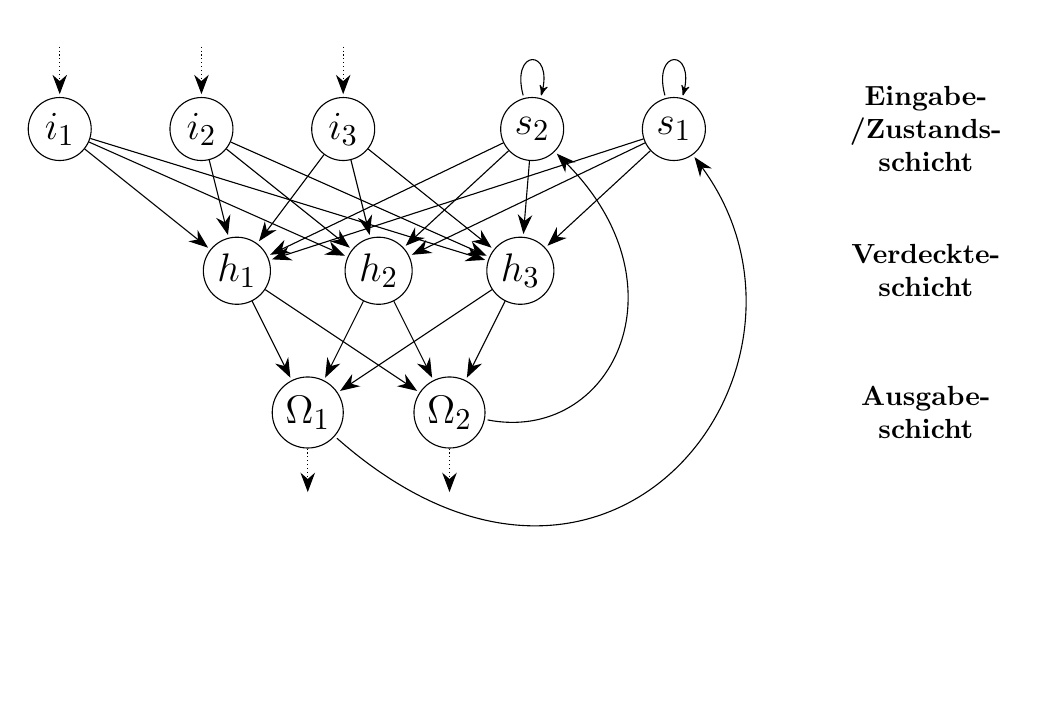
\begin{tikzpicture}[>=stealth', node distance=\layersep cm, shorten >=1pt]
        \def\layersep{1.8}            % vertikal distance between the layers
        \def\neuronsep{1.8}         % Horizontal distance between neurons
        \def\dlsize{2}            % distance between node and layer lable
        \def\inout{\layersep*.65}   % Size of in- and output-arrow
        \def\siz{.8}                % neuronsize
        \def\y{5}                   % Start of the most upper layer
        \def\ni{3}                  % Amount of input neurons
        \def\nh{3}                  % Amount of hidden neurons
        \def\no{2}                  % Amount of output neurons
        \tikzstyle{neuron}=[circle,draw=black,minimum size=\siz cm,inner sep=2pt]
        \tikzstyle{annot} = [text width=6em, text centered]
        \tikzset{fontscale/.style = {font={\fontsize{#1pt}{#1pt}\selectfont}}}
        \newcommand{\neurono}[2][]{
            \node[neuron,circle split,inner sep=2pt] (#1) at (#2)
                    {\includegraphics[width=0.225cm]{Bilder/Sigma.png} \nodepart{lower} \includegraphics[width=0.225cm]{Bilder/sigma.png}};
        }
        % Draw the input layer nodes
            \foreach \name / \xn in {1,...,\ni}{
                \node[neuron,fontscale=15] (Il-\name) at (\xn*\neuronsep-\neuronsep,\y) {$i_{\xn}$};
                \node[above of=Il-\name, node distance=\inout cm] (Inl-\name) {};
                \draw [->,arrows={-Stealth[length=7pt]},densely dotted] (Inl-\name) edge (Il-\name);
            }
        % Draw the state layer nodes
            \foreach \name / \xn in {2/1,1/2}{
                \node[neuron,fontscale=15] (Sl-\name) at (\xn*\neuronsep-\neuronsep+6,\y) {$s_{\name}$};
            }
        % Draw the hidden layer nodes
            \foreach \name / \xn in {1,...,\nh}{
                \node[neuron] (Hl-\xn) at ({(\ni-1)*\neuronsep/2-\neuronsep/2*(\nh-1)+(\xn-1)*\neuronsep+2.25},\y-\layersep) [fontscale=15] {$h_{\xn}$};
                \node[node distance=\inout cm, below of=Hl-\xn] (Hnl) {};
        % Connect every node in the input/state layer with the hidden layer
                \foreach \source in {1,...,\ni}
                    \draw [->,arrows={-Stealth[length=7pt]}] (Il-\source) edge (Hl-\xn);
             
                \foreach \source in {1,...,2}
                    \draw [->,arrows={-Stealth[length=7pt]}] (Sl-\source) edge (Hl-\xn);    
            }
        % Draw the output layer node
            \foreach \name / \xn in {1,...,\no}{
                \node[neuron] (Ol-\xn) at ({(\ni-1)*\neuronsep/2-\neuronsep/2*(\no-1)+(\xn-1)*\neuronsep+2.25},\y-2*\layersep) [fontscale=15] {$\Omega_{\xn}$};
                ,\y+2*\layersep,
                \node[node distance=\inout cm, below of=Ol-\xn] (Onl) {};
                \draw [->,arrows={-Stealth[length=7pt]},densely dotted] (Ol-\xn) edge (Onl);
        % Connect every node in the hidden/state layer with the output layer
                \foreach \source in {1,...,\nh}
                    \draw [->,arrows={-Stealth[length=7pt]}] (Hl-\source) edge (Ol-\xn);
            }
            \draw[arrows={-Stealth[length=7pt]}, shorten >=1pt, shorten <=1pt] (Ol-2) .. controls (7,1) and  (8,3) .. (Sl-2); 
            \draw[arrows={-Stealth[length=7pt]}, shorten >=1pt, shorten <=1pt] (Ol-1) .. controls (7,-2) and  (10,2) .. (Sl-1);
            \draw[arrows={-Stealth[length=7pt]}, shorten <=1pt] (Sl-1) edge[loop above] ();
            \draw[arrows={-Stealth[length=7pt]}, shorten <=1pt] (Sl-2) edge[loop above] ();
        % Annotate the layers
                \node[annot] (il) at (11,5) {\textbf{Eingabe-/Zustands- schicht}};
                \node[annot,below of=il] (hl) {\textbf{Verdeckte- schicht}};
                \node[annot,below of=hl] {\textbf{Ausgabe- schicht}};
    \end{tikzpicture}
    }
    \caption{Jordannetz mit drei Eingabeneuronen $i$, zwei Zustandsneuronen $s$, drei verdeckten Neuronen $h$ und zwei Ausgabeneuronen $\Omega$.}
    \label{fig:Jordannetz}
\end{figure}

Diese beiden Netzwerke ähneln sich sehr in ihrer Beschaffenheit und werden daher zusammen vorgestellt. Mehr noch stellte unter anderen die Arbeit von \citet{Jordan1986} die Grundlage für die Veröffentlichung von \citet{Elman1990}. Die Modelle die in diesen Arbeiten vorgestellt werden zählen zu den rückgekoppelten (engl.: recurrent) neuronalen Netzen. Die Grundform bildet hierbei ein Feed-Forward Netz wie beispielsweise das MLP. Zusätzlich gibt es sogenannte Kontext bzw. Zustandsneuronen (engl.: context/state neurons). Diese Bilden im übertragenden Sinne eine weitere verdeckte Schicht in dem Sinne das sie keine Kommunikation mit der \glqq Außenwelt\grqq~besitzt. Diese Neuronen zeichnen sich dadurch aus, dass entweder die Outputneuronen (Jordan Netz) bzw. die Neuronen der Verdecktenschicht (Elamn Netz) eine Rückkopplung zu ihnen aufweisen. Zusätzlich weisen diese Neuronen eine Eigenrückkoplung auf (\farbig{sihe Abbildung ??}). \todo{tiefer ins detail gehen}

\begin{figure}[!htb]
    \centering
    %---------------------------------------------------------------
        %% Elmannetz
        %-----------------------------------------
        \input{Bilder/Netzwerke/Elman.tex}
    \caption{Elmannetz mit drei Eingabeneuronen $i$, drei Kontextneuronen $k$, drei verdeckten Neuronen $h$ und zwei Ausgabeneuronen $\Omega$.}
    \label{fig:Elman}
\end{figure}

Durch die zusätzliche Rückkopplung bekommt das Netzwerk ein zeitliches Gedächtnis, indem der wert des vorherigen Durchlaufes zwischengespeichert und für die Berechnung des nächsten Wertes berücksichtigt wird. Durch die Eigenrückkopplung kann die zeitliche Ausdehnung des Gedächtises kontrolliert werden. Zum Trainieren der Neuronalen Netze kann ebenfalls der Backpropagationalgorithmus angewandt werden, wobei die Eigenrückkopplungsrate während der Trainingsphase der Gewichte konstant gehalten werden muss. Hierzu wurden in der Literatur\,\citef{Pham1999} Modifikationen am Netzwerk und am Lernalgorythmus vorgestellt, um das Backpropagationverfahren auch auf die Kontextneuronen anwenden zu können.


\subsubsection{Hopfieldnetze}%\\
\begin{figure}[!htb]
    \centering
    %---------------------------------------------------------------
        %% Hopfieldnetz
        %-----------------------------------------
            %---------------------------------------------------------------
        %% Hopfieldnetz
        %-----------------------------------------
        %% linkes Bild
        \begin{tikzpicture}[ node distance=\layersep cm, shorten >=1pt]
        \def\layersep{2}            % vertikal distance between the layers
        \def\neuronsep{2}           % Horizontal distance between neurons
        \def\dlsize{2}              % distance between node and layer lable
        \def\inout{\layersep*.65}   % Size of in- and output-arrow
        \def\siz{.8}                % neuronsize
        \def\y{3}                   % Start of the most upper layer
        \def\no{3}                  % Amount of output neurons
        \tikzstyle{neuron}=[circle,draw=black,minimum size=\siz cm,inner sep=2pt]
        \tikzstyle{annot} = [text width=6em, text centered]
        \tikzset{fontscale/.style = {font={\fontsize{#1pt}{#1pt}\selectfont}}}
        \tikzset{
                ident/.pic={
                    \ifthenelse{\equal{#1}{1} \OR \equal{#1}{3}}{
                        \draw[semithick,arrows={-Latex[open]}] (0,-\siz/3) -- (0,\siz/3);
                    }{
                        \draw[semithick,arrows={Latex[open]-}] (0,-\siz/3) -- (0,\siz/3);
                    }
                    
                }
            }
        % Draw the left output layer node
            \foreach \xn in {1,...,\no}{
                \node[neuron] (Ol-\xn) at (\xn*\neuronsep-\neuronsep,\y) [fontscale=15] {$\Omega_{\xn}$};
                \node[above of=Ol-\xn, node distance=\inout cm] (Onla-\xn) {};
                \node[below of=Ol-\xn, node distance=\inout cm] (Onlb-\xn) {};
                \draw[arrows={-Stealth[length=7pt]},densely dotted] (Onla-\xn) edge (Ol-\xn);
                \draw[arrows={-Stealth[length=7pt]},densely dotted] (Ol-\xn) edge (Onlb-\xn);
            }
        % Connect every node in the output layer
            \pgfmathsetmacro{\nom}{\no - 1}
               \foreach \xn in {1,...,\nom}{
                    \pgfmathtruncatemacro{\xnp}{\xn + 1}
                    \draw[arrows={Stealth[length=7pt]-Stealth[length=7pt]},shorten <=1pt] (Ol-\xn) edge[bend right=45] (Ol-\xnp);
                        \node[fill=white,inner sep=.1pt,fontscale=10] at ($(Ol-\xnp)!.4+.1!(Ol-\xn)+(0,-0.65)$) {$w_{\xnp,\xn}$};
                }
            \draw[arrows={Stealth[length=7pt]-Stealth[length=7pt]},shorten <=1pt] (Ol-1) edge[bend right=65] (Ol-\no);
            \node[fill=white,inner sep=.1pt,fontscale=10] at ($(Ol-1)!.4+.1!(Ol-\no)+(0,-1.45)$) {$w_{1,\no}$};
        % Annotate the layers
               \node[annot,right of=Ol-\no, node distance=\dlsize cm] (ol) {\textbf{Eingabe-/Ausgabe- schicht}};
        %-----------------------------------------
        %% rechtes Bild
        % Draw the right output layer nodes
            \foreach \xn in {1,...,\no}{
                \node[neuron,right of=ol] (Or-\xn) at ($(ol)+(\xn*\neuronsep-\neuronsep,0)$) {};
                \pic at (Or-\xn) {ident=\xn};
            }
        % Draw the right upper and lower output layer nodes
            \foreach \xn in {1,...,2}{
                \node[neuron] (Orb-\xn) at ($(Or-2)+({\neuronsep/2-\neuronsep/2*(\no-1)+(\xn-1)*\neuronsep},-\layersep)$) {};
                \node[neuron] (Ora-\xn) at ($(Or-2)+({\neuronsep/2-\neuronsep/2*(\no-1)+(\xn-1)*\neuronsep},\layersep)$) {};
                \pic at (Orb-\xn) {ident=\xn};
                \pic at (Ora-\xn) {ident=\xn};
            }    
        % Connect every node in the right output layer
            \foreach \xn in {1,...,\nom}{
                \pgfmathtruncatemacro{\xnp}{\xn + 1}
                \draw[arrows={Stealth[length=7pt]-Stealth[length=7pt]},shorten <=1pt] (Or-\xn) edge (Or-\xnp);
            }    
            \foreach \xn in {1,...,\no}{
                \foreach \xp in {1,2}{
                    \draw[arrows={Stealth[length=7pt]-Stealth[length=7pt]},shorten <=1pt] (Or-\xn) edge (Ora-\xp);
                    \draw[arrows={Stealth[length=7pt]-Stealth[length=7pt]},shorten <=1pt] (Or-\xn) edge (Orb-\xp);
                }
            }
            \draw[arrows={Stealth[length=7pt]-Stealth[length=7pt]},shorten <=1pt] (Orb-1) edge[bend right=30] (Ora-2);
            \draw[arrows={Stealth[length=7pt]-Stealth[length=7pt]},shorten <=1pt] (Orb-2) edge[bend left=30] (Ora-1);
            \draw[arrows={Stealth[length=7pt]-Stealth[length=7pt]},shorten <=1pt] (Or-3)  edge[bend right=35] (Or-1);
            \node[fill=white,inner sep=1pt,fontscale=10] at ($(Or-1)+({(\no-1)*\neuronsep/2},\layersep*.5)$) {$\dots\, w_{i,j}\,\dots$};
            \node[fill=white,inner sep=1pt,fontscale=10] at ($(Or-1)+({(\no-1)*\neuronsep/2},-\layersep*.5)$) {$\dots\, w_{i,j}\,\dots$};
        \end{tikzpicture}
    \caption{Hopfieldnetz mit drei Neuronen und den zugehörigen Gewichten $w$ in der Seitenansicht auf der linken Seite. Die rechte Seite zeigt das gleiche Netzwerk mit den zugehörigen neuronalen Zustand in der Draufsicht.\,\protect\footnotemark{}}
    \label{fig:Hopfield}
\end{figure}
\addtocounter{footnote}{-1}     %  -1 mal die Gesamtanzahl an Fußnoten in der wrapfigure
\addtocounter{Hfootnote}{-1}    % -1 times total number of footnote(mark)s in the wrapfigure
\wrapfigfoot\footnotetext{Die rechte Darstellung des Hopfieldnetzes in \autoref{fig:Hopfield} wurde der Abbildung 8.1 aus \citet[136]{dkriesel07} nachempfunden.}
Das Hopfield Netz benannt nach seinem Entwickler zählt zu den rückgekoppelten Netzen. \citet{HOPFIELD1986} stellte ein Netzwerk vor, dass dem Verhalten von Teilchen in einem Magnetfeld nachempfunden ist.\,\citef[135]{dkriesel07} Die Neuronen dieses Netzes sind untereinander vollverknüpft haben aber keine Verbindung zu sich selbst. Weiterhin dient die Heavisidefunktion (\autoref{fig:funktion} links) mit den möglichen Zuständen von $1$ und $-1$ als Aktivierungsfunktion und die Verbindung unter den Neuronen ist gewichtet. Die Gewichte können positiv (je höher der Wert desto mehr tendieren die Neuronen zu gleichem Zustand), negativ (je größer der Betrag des Gewichtes desto mehr streben die Neuronen zu unterschiedlichen Werten) oder null (Neuronen beeinflussen sich gegenseitig nicht) sein. Analogiekonform kann der Zustand der Neuronen auch als Spinn (Drehwinkel) der Teilchen betrachtet werden. Die Eingabe des Netzwerks geschieht durch die Festlegung der Neuronenzustände. Trainiert wird das Netz indem die Trainigsbeispiele eingegeben werden und die Gewichte nach der Beziehung zueinander verändert werden. Am Ende der Trainingsphase haben die Gewichte einen hohen positiven Wert bei denen die Neuronen oft den gleichen Zustand inne gehabt haben und für hohe negative Gewichte gilt der umgekehrte Fall. Das Netzwerk sucht nach der Eingabe von Informationen selbstständig den energetisch geringsten Zustand zum betreffenden Eingabemuster. Dies geschieht unter Berücksichtigung der Gewichte und Veränderung der Spins. Hierbei wird der Zustand der Neuronen einzeln verändert, wobei das zu verändernde Neuron zufällig ausgewählt wird. Wenn die Spins sich nicht mehr ändern ist der energetisch geringste Zustand erreicht. Die resultierende Spinnverteilung der Neuronen ergibt dann die Ausgabe des Netzwerks. Hauptsächlich wir dieses Netzwerk zur Mustererkennung eingesetzt. Das zu erkennende Muster dient als Trainingsbeispiel und das Netzwerk ist dann in der Lage das gleiche Muster in verrauschter Form wiederzuerkennen.


\subsubsection{Adaptive Resonance Theory (ART)}%\\
\begin{figure}[!htb]
    \centering
    %---------------------------------------------------------------
        %% ART
        %-----------------------------------------
        %% Compiler: XeLaTeX

\documentclass[tikz,border=0pt]{standalone}%
\usepackage{tikz-cd}
\usetikzlibrary{arrows}

\begin{document}

%---------------------------ART-------------------------------------------------------------------------------------------%
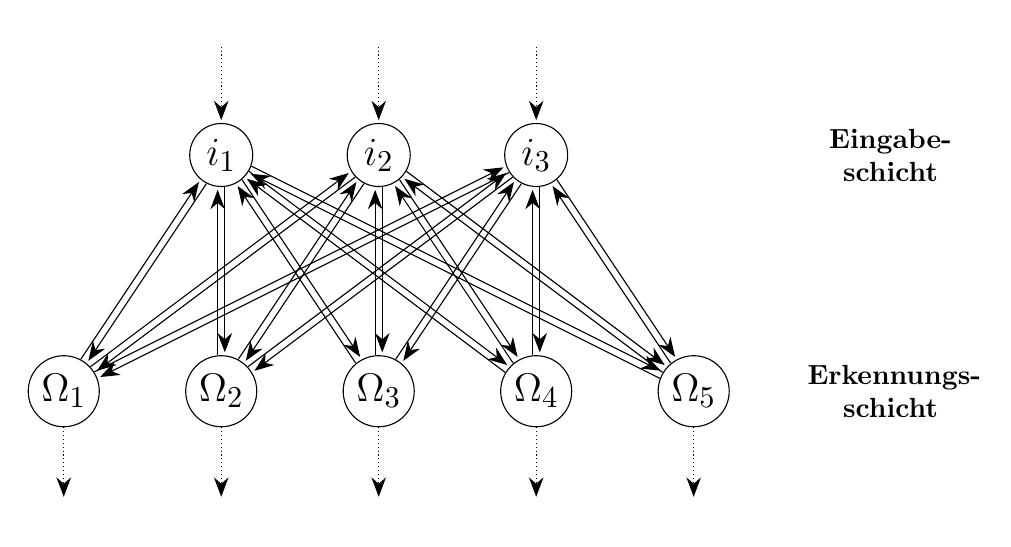
\begin{tikzpicture}[>=stealth', node distance=\layersep cm, shorten >=1pt]

        \def\layersep{3}            % vertikal distance between the layers
        \def\neuronsep{2}           % Horizontal distance between neurons
        \def\dlsize{2.5}            % distance between node and layer lable
        \def\inout{\layersep*.5}    % Size of in- and output-arrow
        \def\siz{.8}                % neuronsize
        \def\y{3}                   % Start of the most upper layer
        \def\ni{3}                  % Amount of input neurons
        \def\no{5}                  % Amount of output neurons
        \tikzstyle{neuron}=[circle,draw=black,minimum size=\siz cm,inner sep=2pt]
        \tikzstyle{annot} = [text width=6em, text centered]
        \tikzset{fontscale/.style = {font={\fontsize{#1pt}{#1pt}\selectfont}}}
        \tikzset{
            shift left/.style ={commutative diagrams/shift left={#1}},
            shift right/.style={commutative diagrams/shift right={#1}}
        }
        
        % Draw the left input layer nodes
            \foreach \xn in {1,...,\ni}{
                \node[neuron,fontscale=15] (Il-\xn) at (\xn*\neuronsep-\neuronsep,\y) {$i_{\xn}$};
                \node[above of=Il-\xn, node distance=\inout cm] (Inl-\xn) {};
                \draw [arrows={-Stealth[length=7pt]},densely dotted] (Inl-\xn) edge (Il-\xn);
            }
        % Draw the output layer node
            \foreach \xn in {1,...,\no}{
                \node[neuron] (Ol-\xn) at ({(\ni-1)*\neuronsep/2-\neuronsep/2*(\no-1)+(\xn-1)*\neuronsep},\y-\layersep) [fontscale=15] {$\Omega_{\xn}$};
                \node[node distance=\inout cm, below of=Ol-\xn] (Onl) {};
                \draw [->,arrows={-Stealth[length=7pt]},densely dotted] (Ol-\xn) edge (Onl);
        % Connect every node in the input layer with the output layer                
            \foreach \source in {1,...,\ni}{
                \draw [->,arrows={-Stealth[length=7pt]}, shift left=.3ex] (Il-\source) edge (Ol-\xn);
                \draw [->,arrows={-Stealth[length=7pt]}, shift left=.3ex] (Ol-\xn) edge (Il-\source);
                }}
                
        % Annotate the layers
                \node[annot,right of=Ol-\no, node distance=\dlsize cm] (ol) {\textbf{Erkennungs- schicht}};
                \node[annot,above of=ol] (il) {\textbf{Eingabe- schicht}};
                
        \end{tikzpicture}
\end{document}
    \caption{Vereinfachte Darstellung des ART-Netzes. Mit der Eingabeschicht oben und der Erkennungsschicht unten. Die Steuerungs- und Kontrollneuronen wurde der Übersicht halber nicht dargestellt.\,\protect\footnotemark{}}
    \label{fig:ART}
\end{figure}
\addtocounter{footnote}{-1}     %  -1 mal die Gesamtanzahl an Fußnoten in der wrapfigure
\addtocounter{Hfootnote}{-1}    %  -1 times total number of footnote(mark)s in the wrapfigure
\wrapfigfoot\footnotetext{Die Darstellung des ART-Netzes in \autoref{fig:ART} wurde der Abbildung 11.1 aus \citet[174]{dkriesel07} nachempfunden.}
%\todo{Grafik Buch:Fausett-S.233}
Den Grundstein für die Theorie des ART Netzes legte \citet{Grossberg1973} und es zählt zu den rückgekoppelten Netzen, welche unbeaufsichtigt lernen. Das ART1, dass in diesem Kapitel näher erläutert wird, wurde von \citet{Carpenter1987} vorgestellt. Dieses Netzwerk wurde mit dem Hintergedanken entwickelt, dass die bis dato vorgestellten Netzwerktypen Schwierigkeiten gehabt haben neue Informationen zu bestehenden hinzuzufügen ohne die bisherigen Informationen zu \glqq vergessen\grqq . Daher ist das ART Netzwerk in der Lage binäre Muster in Klassen einzuteilen wobei es zusätzlich neue Klassen finden kann. Aufgebaut ist das Netzwerk aus zwei Schichten. Nämlich der Eingabeschicht und der Erkennungsschicht, wobei die Erkennungsschicht auch für die augabe der Informationen zuständig ist. Beide Schichten sind untereinander vollverknüpft. Hierbei wird der Informationsfluss von den Eingabeneuronen zu den Erkennungsneuronen hin als Bottom-Up Verbindung bezeichnet und der rückwärtige Informationsfluss als Top-Down Verbindung. Anfänglich wird das Netzwerk mit unbestimmten Gewichten initialisiert. Darauffolgend werden binäre Eingaben von der gleichnamigen Schicht an die Erkennungsschicht weitergegeben wo nach dem Winnter-Takes-All Schema das Neuron mit der größten Aktivierung ausgewählt wird. Nun werden die Gewichte der Bottom-Up Verbindung die zum \glqq Gewinnerneuron\grqq~führen erhöht. Hiermit wird die Klassenzugehörigkeit des Eingabemusters verstärkt. Die Aktivität der Erkennungsschicht wird anschließend über die Top-Down Verbindung an die Eingabeschicht zurückgegeben. Hier werden ebenfalls nur die Gewichte trainiert die vom \glqq Gewinnerneuron\grqq~zur Eingabeschicht führen. Die \glqq Aktiviät\grqq~wird so von einer Schicht an die andere und wieder zurück geleitet wodurch der Begriff der Resonanz geprägt wird.\\
Es kommt vor, dass mehrere Neuronen der Erkennungsschicht eine gleiche Aktivität aufweisen. In diesem Fall erzeugt ein Steuerungsneuron ein zusätzliches Ausgabeneuron und ordnet diesem das aktuelle Muster zu. Bei der Eingabe ähnlicher Muster stellt sich die Frage wann ein Neuron aktiv werden darf und wann gelernt wird. Hierfür existieren im ART-Netz Kontrollneurone welche diese Spezialfälle durch verschiedene mathematische Regeln behandeln.\\
Der Vorteil dieses Netzes ist nicht nur, dass es die Eingabe in Klassen einordnen kann sondern durch die Aktivierung des des Ausgabeneurons auch verraten kann wie ein typischer Vertreter dieser Klasse aussieht. Als größter Kritikpunkt gilt hier die Notwendigkeit von Spezialfallunterscheidungen die durch diverse \glqq IF-Abfragen\grqq~abgefangen werden müssen.\,\citef[173 ff]{dkriesel07}\\
Wie zu Beginn dieses Unterkapitels durch ART1 angedeutet gibt es nicht das ART-Netz sondern eine Vielzahl von Weiterentwicklungen und Verbesserungen. Einige erlauben neben binären auch kontinuierliche Eingaben, andere bieten eine höhere Lerngeschwindigkeit.\,\footnote{Vgl. \citet[C2.2:1 ff]{Fiesler96} und \citet[89 ff]{Gurney1997}.} 

%Eine genauere Beschreibung und Übersicht der ART-Familie geben \citet[C2.2:1 ff]{Fiesler96} und \citet[89 ff]{Gurney1997}.


\subsubsection{Cascade-Correlation Netze (CCNN/RCC)}%\\
\begin{figure}[!htb]
    %\centering
    %---------------------------------------------------------------
        %% CCNN
        %-----------------------------------------
        \includestandalone[mode=image|tex,trim=0pt 0pt 0pt .8cm,clip]{Bilder/Netzwerke/CCNN}
    \caption{\farbig{caption einfügen}.\,\protect\footnotemark{}}
    \label{fig:ccnn}
\end{figure}
\addtocounter{footnote}{-1}     %  -1 mal die Gesamtanzahl an Fußnoten in der wrapfigure
\addtocounter{Hfootnote}{-1}    % -1 times total number of footnote(mark)s in the wrapfigure
\wrapfigfoot\footnotetext{Die \autoref{fig:ccnn} wurde der Figure 2 aus \citet[3]{Balazs2009} nachempfunden.}

Das Cascade-Correlation Modell wurde als überwacht lernendes Feed-Foreward Netzwerk von \citet{Fahlman1990} vorgestellt. Die Idee hinter CCNN ist, dass es zunächst mit einem SLP initialisiert und angelernt wird und solange nach bedarf selbstständig neue Neuronen hinzufügen kann bis der Gewünschte Fehlerterm erreicht ist.\\
Genauer gesagt wird nach der initialisierung des SLP das Netzwerk trainiert und der Fehlerterm zwischen der Ausgabe und der Lösung des Trainingsbeispiels beobachtet. Falls nicht der gewünschte Wert erreicht wird fügt der Algorythmus ein verdecktes Neuron (das sogenannte Kandidatneuron) hinzu und trainiert dieses. Hier liegt auch der Unterschied zwischen den anderen Mehrschichtnetzen. Wird ein Kandidatneuron hinzugefügt so werden zunächst gewichtete Verbindungen zu den bisherigen Neuronen (hierzu zählen die Eingabe- wie auch die verdeckten Neuronen) gebildet mit Ausnahme der Ausgabeneuronen. Die Gewichte des neu erzeugten Neurons werden nun mit einem Gradientenabstiegsverfahren trainiert, wobei die Gewichte der anderen Neuronen eingefroren werden. Nach einem im Vorfeld festgelegten Fehlerreduktionsterm wird das Training des Kandidatneurons beendet. Als nächstes wird das Kandidatneuron mit einer Gewichteten Verbindung ebenfalls mit den Ausgabeneurone verbunden. Nun werden alle Gewichte mit Ausnahme der Gewichte Der Ausgabeneuronen eingefrohren und mit Hilfe eines Lernalgorithmus für Einschichtige Netze (beispielsweise mit der Deltaregel) trainiert.\\
\citet{Fahlman1990} beschreiben auch die Möglichkeit mehrere Kadidatneurone gleichzeitig zu trainieren und das erfolgversprechendste in das Netzwerk einzubinden. Hierdurch wird die Moglichkeit reduziert in einem lokalen Minimum stecken zu bleiben. Zusätzlich können die Kandidatneuronen unterschiedliche Aktivierungsfunktionen beinhalten und das so entstehende inhomogene Netzwerk kann zu eleganteren Lösungen führen im vergleich zu homogenen Netzwerken.\\
Der Vorteil dieses Netzwerkes besteht neben des sehr schnellen Lernvorgangs darin, dass das Netzwerk je nach Problemstellung die eigene Größe und Topologie selbst bestimmen kann. \citet{Balazs2009} gibt an, dass die CCNN aber auch leicht Überangepasst (engl.: overfit) werden können.\\
\todo{Grafik}
\citet{Fahlman1991} stellte das rückgekoppeles Cascade-Correlation Netz (RCC) vor. Dieses Netzwerk (dargestellt in \farbig{Abbildung ??}) ist inspiriert durch das Elamn Netz. Aber anstatt Verbindungen zu Neuronen vorherigen Schichten zu bilden, welches das CCNN Konzept verletzen würde, besitzen die verdeckten Neuronen und die Kandidatneurone eine gewichtete Eigenrückkopplung. Mit dieser Änderung ist das Netz in der Lage, neben den Eigenschaften des CCNN, Muster in Zeitdiskreten Daten zu erkennen. Wie aber \citet{Kirschninga1995} feststellen hat die Grundform des RCC probleme große Gruppen von Mustern mit unterschiedlichen Eigenschaften zu erkennen. Bei einer großen Datenlage scheint das Netzwerk sogar zuvor gelernte Muster zu vergessen.  




%\newpage
\subsection{Gegenüberstellung der Netzwerke}
%In diesem Abschnitt erfolgt eine Zusammenfassung der Eigenschaften der vorgestellten Modelle.

Vor dem Hintergrund der zuvor vorgestellten Charakterisierung und Anwendungsgebiete der NN erfolgt in \autoref{tab:ann_modell} eine Gegenüberstellung der vorgestellten Modelle. Es wird an dieser Stelle nochmal darauf hingewiesen, dass die Kategorisierung der Anwendungen nicht klar umgrenzt sind und die Zuordnung der Anwendungsgebiete als Tendenz angesehen werden sollte.

\begin{table}[h]
%\centering
\caption{Gegenüberstellung vorgestellter Modelle}
\label{tab:ann_modell}
\begin{tabularx}{\textwidth}{llZZ}
\toprule
Modell          &  Neuronaleverbindung   & Lernverfahren          & Anwendung           \\
\midrule
MLP             & FF        & überwacht         & K-r, AM-h, AM-a                       \\
RBF             & FF        & überwacht         & K-nn\,\protect\footnotemark{}, AM-h   \\
SOM             & R-l       & unüberwacht       & K-nn, KO, AM-h                        \\
GRNN            & FF        & unüberwacht       & K-r                                   \\
Jordan/Elman    & R-i       & überwacht         & K-r, AM-h                             \\
Hopfield        & R-v       & unüberwacht       & AM-a, KO                              \\
ART             & R-v       & unüberwacht       & K-nn, AM-h                            \\
CCNN            & FF        & überwacht         & K-r, AM-h                             \\
RCC             & R-d       & überwacht         & K-r, AM-h                             \\


\bottomrule
\end{tabularx}
\farbig{\fontsize{10pt}{10.5pt}\selectfont Abkürzungen ausschreiben Bsp.: K-r:Klassifikation durch Regression, K-nn:Klassifikation durch nächster-Nachbar}
\end{table}
\addtocounter{footnote}{-1}     %  -1 mal die Gesamtanzahl an Fußnoten in der wrapfigure
\addtocounter{Hfootnote}{-1}    % -1 times total number of footnote(mark)s in the wrapfigure
\wrapfigfoot\footnotetext{Vgl. \citet[F1.2:4]{Fiesler96}.}


\begin{comment} %--------DAS IST EIN KOMMENTAR----ANFANG----------%


In diesem Abschnitt erfolgt eine Bewertung der vorgestellten neuronalen Netzwerke vor dem Hintergrund der Anwendbarkeit auf die Vorhersage von Strommarktpreisen.

\vspace{1cm}


%-------------------------------------------
%% Inhalt für Gegenüberstellungstabelle
\newcommand{\vergleich}[2][1]{%
%------------------ SLP ------------------%
        \ifthenelse{\equal{#1}{slp}}{%
            \ifthenelse{\equal{#2}{v}}{% Vorteil
                %\begin{itemize}%
                    %\item%
                    \tabitem{%
                        Können Funktionen approximieren}
                    %\item%
                    \tabitem{%
                        Einfacher Aufbau}
                %\end{itemize}%
            }{}%
            \ifthenelse{\equal{#2}{n}}{% Nachteil
                \begin{itemize}%
                    \item%
                        Kann nur linear separierbare Daten repräsentieren und somit kein XOR geschweige denn komplexere Funktionen
                \end{itemize}%
            }{}%
        }{}%
%------------------ MLP ------------------%
        \ifthenelse{\equal{#1}{mlp}}{%
            \ifthenelse{\equal{#2}{v}}{% Vorteil
                \begin{itemize}%
                    \item%
                        Beliebig genaue Approximation von Funktionen
                    \item%
                        Höhere Anzahl an Eingabeneuronen hat geringen/keinen Einfluss auf Anzahl der versteckten Neuronen
                \end{itemize}%
            }{}%
            \ifthenelse{\equal{#2}{n}}{% Nachteil
                \begin{itemize}%
                    \item%
                        Eine höhere Anzahl an Ausgabeneuronen führt bei Backpropagation zu einer höheren Lerndauer
                \end{itemize}%
            }{}%
            \ifthenelse{\equal{#2}{v-n}}{% Vor-/Nachteil
                \begin{itemize}%
                    \item%
                        Extrapolationsfähig - Kann zwischen approximierter Funktion und möglichen Ausreißern extrapolieren. Es bleibt dem Anwender überlassen ob das Ergebnis vertrauenswürdig ist.
                    \item%
                        Ein Ausfall von Gewichten/Neuronen nach dem Lernvorgang führt zu einem globalen Berechnungsfehler
                \end{itemize}%
            }{}%
        }{}%
%------------------ RBF ------------------%
        \ifthenelse{\equal{#1}{rbf}}{%
            \ifthenelse{\equal{#2}{v}}{% Vorteil
                \begin{itemize}
                    \item
                        Beliebig genaue Approximation von Funktionen
                    \item
                        Höhere Anzahl an Ausgabeneuronen hat geringen Einfluss auf Lerngeschwindigkeit
                \end{itemize}
            }{}%
            \ifthenelse{\equal{#2}{n}}{% Nachteil
                \begin{itemize}
                    \item
                        Exponentieller Anstieg der RBF-Neuronen bei steigender Anzahl an Eingabeneuronen bedingt einen höheren Speicher- und Rechenaufwand
                    \item
                        Positionierung der Zentren hat großen Einfluss auf die Lerngeschwindigkeit und Approximationsgenauigkeit
                \end{itemize}
            }{}%
            \ifthenelse{\equal{#2}{v-n}}{% Vor-/Nachteil
                \begin{itemize}%
                    \item%
                        Nicht Extrapolationsfähig - Eingabewerte weit weg von den Zentren führen zu dem Ergebniss 0. Das Netzwerk ist in der Lage zu sagen dass es auf die Eingabeinformation keine Antwort geben kann.
                    \item%
                        Ein Ausfall von Gewichten/Neuronen nach dem Lernvorgang beeinflusst weite Teile des Netzes nicht - Eine Stelle des Outputs ist aber sehr betroffen da hier direkt eine Funktion fehlt - Dies führt daher zu einem lokalen Fehler 
                \end{itemize}%
            }{}%
        }{}%
%------------------ SOM ------------------%
        \ifthenelse{\equal{#1}{som}}{%
            \ifthenelse{\equal{#2}{v}}{% Vorteil
                \begin{itemize}
                    \item
                        Ermöglicht Nachbarschaftsbeziehungen in Daten zu finden
                \end{itemize}
            }{}%
            \ifthenelse{\equal{#2}{n}}{% Nachteil
                \begin{itemize}
                    \item
                        Kein Funktionsapproximator
                    \item
                        Die Wahl der Verknüpfung der Ausgabeneuronen hat großen Einfluss auf die Darstellungsfähigkeit des Netzwerks
                \end{itemize}
            }{}%
        }{}%
}

\begin{center}
\definecolor{tableHeader}{RGB}{255, 255, 255}
\definecolor{tableLineOne}{RGB}{255, 255, 255}
\definecolor{tableLineTwo}{RGB}{250, 250, 250}

\newcommand{\tabitem}[1]{~~\llap{\textbullet}~~#1\newline}

\newcommand{\tableHeaderStyle}{
    %
    \rowfont{\leavevmode\color{black}\bfseries}
    %\rowfont{\color{black}\bfseries}
    \rowcolor{tableHeader}
}

\taburowcolors[2] 2{tableLineOne .. tableLineTwo}
\tabulinesep =^4mm_1mm
\extrarowsep=1mm
%\everyrow{\tabucline[.4mm  white]{}}

%\begin{longtabu} to \textwidth { X[c, 1.5] X[4] X[4] X[4]}%
%        \tableHeaderStyle%
%        \toprule[1.5pt]
%        Netzwerk                                & Vorteil            & Nachteil           & Neutral                 \\
%        \midrule
%        Sinle Layer Perceptron \textbf{(SLP)}   & \vergleich[slp]{v} & \vergleich[slp]{n} &                         \\
%        Multi Layer Perceptron \textbf{(MLP)}   & \vergleich[mlp]{v} & \vergleich[mlp]{n} & \vergleich[mlp]{v-n}    \\
%        Radiale Basisfunktionen \textbf{(RBF)}  & \vergleich[rbf]{v} & \vergleich[rbf]{n} & \vergleich[rbf]{v-n}    \\
        %\hline\hline
%        Self Organizing Maps \textbf{(SOM)}     & \vergleich[som]{v} & \vergleich[som]{n} &                         \\
%\end{longtabu}    
    
\end{center}
%--------------------------------------------------------------------------------------------------------------------------------------------------%


%-------------------------------------------
%% Inhalt für Gegenüberstellungstabelle
\newcommand{\vergleich}[3][1]{%
%------------------ SLP ------------------%
        \ifthenelse{\equal{#1}{slp}}{%
            \ifthenelse{\equal{#2}{v}}{% Vorteil
                %\begin{easylist}
                    \tabitem{% 
                        Können Funktionen approximieren}{#3}%
                    \vspace{0.4cm}
                    \tabitem{% 
                        Einfacher Aufbau}{#3}%
                %\end{easylist}%
            }{}%
            \ifthenelse{\equal{#2}{n}}{% Nachteil
                %\begin{easylist}%
                    %@%
                    \tabitem{%
                        Kann nur linear separierbare Daten repräsentieren und somit kein XOR geschweige denn komplexere Funktionen}{#3}%
                %\end{easylist}%
            }{}%
        }{}%
%------------------ MLP ------------------%
        \ifthenelse{\equal{#1}{mlp}}{%
            \ifthenelse{\equal{#2}{v}}{% Vorteil
                %\begin{easylist}%
                    %@%
                    \tabitem{%
                        Beliebig genaue Approximation von Funktionen}{#3}%
                    \vspace{0.4cm}
                    %@%
                    \tabitem{%
                        Höhere Anzahl an Eingabeneuronen hat geringen/keinen Einfluss auf Anzahl der versteckten Neuronen}{#3}%
                %\end{easylist}%
            }{}%
            \ifthenelse{\equal{#2}{n}}{% Nachteil
                %\begin{easylist}%
                    %@%
                    \tabitem{%
                        Eine höhere Anzahl an Ausgabeneuronen führt bei Backpropagation zu einer höheren Lerndauer}{#3}%
                %\end{easylist}%
            }{}%
            \ifthenelse{\equal{#2}{v-n}}{% Vor-/Nachteil
                %\begin{easylist}%
                    %@%
                    \tabitem{%
                        Extrapolationsfähig: Kann zwischen approximierter Funktion und möglichen Ausreißern extrapolieren. Es bleibt dem Anwender überlassen ob das Ergebnis vertrauenswürdig ist}{#3}%
                    %\vspace{0.4cm}
                    %@%
                    %\tabitem{%
                    %    Ein Ausfall von Gewichten/Neuronen nach dem Lernvorgang führt zu einem globalen Berechnungsfehler}{#3}%
                %\end{easylist}%
            }{}%
        }{}%
%------------------ RBF ------------------%
        \ifthenelse{\equal{#1}{rbf}}{%
            \ifthenelse{\equal{#2}{v}}{% Vorteil
                %\begin{easylist}%
                    %@%
                    \tabitem{%
                        Beliebig genaue Approximation von Funktionen}{#3}%
                    \vspace{0.4cm}
                    %@%
                    \tabitem{%
                        Höhere Anzahl an Ausgabeneuronen hat geringen Einfluss auf Lerngeschwindigkeit}{#3}%
                %\end{easylist}%
            }{}%
            \ifthenelse{\equal{#2}{n}}{% Nachteil
                %\begin{easylist}%
                    %@%
                    \tabitem{%
                        Exponentieller Anstieg der RBF-Neuronen bei steigender Anzahl an Eingabeneuronen bedingt einen höheren Speicher- und Rechenaufwand}{#3}%
                    \vspace{0.4cm}
                    %@%
                    \tabitem{%
                        Positionierung der Zentren hat großen Einfluss auf die Lerngeschwindigkeit und Approximationsgenauigkeit}{#3}%
                %\end{easylist}%
            }{}%
            \ifthenelse{\equal{#2}{v-n}}{% Vor-/Nachteil
                %\begin{easylist}%
                    %@%
                    \tabitem{%
                        Nicht Extrapolationsfähig: Eingabewerte weit weg von den Zentren führen zu dem Ergebniss 0. Das Netzwerk ist in der Lage zu sagen dass es auf die Eingabeinformation keine Antwort geben kann}{#3}%
                    %\vspace{0.4cm}
                    %@%
                    %\tabitem{%
                    %    Ein Ausfall von Gewichten/Neuronen nach dem Lernvorgang beeinflusst weite Teile des Netzes nicht~-- Eine Stelle des Outputs ist aber sehr betroffen da hier direkt eine Funktion fehlt~-- Dies führt daher zu einem lokalen Fehler}{#3}%
                %\end{easylist}%
            }{}%
        }{}%
%------------------ SOM ------------------%
        \ifthenelse{\equal{#1}{som}}{%
            \ifthenelse{\equal{#2}{v}}{% Vorteil
                %\begin{easylist}%
                    %@%
                    \tabitem{%
                        Ermöglicht Nachbarschaftsbeziehungen in Daten zu finden}{#3}%
                %\end{easylist}%
            }{}%
            \ifthenelse{\equal{#2}{n}}{% Nachteil
                %\begin{easylist}%
                    %@%
                    \tabitem{%
                        Kein Funktionsapproximator}{#3}%
                    \vspace{0.4cm}
                    %@%
                    \tabitem{%
                        Die Wahl der Verknüpfung der Ausgabeneuronen hat großen Einfluss auf die Darstellungsfähigkeit des Netzwerks}{#3}%
                %\end{easylist}%
            }{}%
        }{}%
}

\newcommand{\tabitem}[2]{\textbullet~~\begin{minipage}[t]{#2\textwidth}\raggedright #1\end{minipage}}

\begin{tabularx}{\linewidth}{>{\setlength\hsize{.5\hsize}}X @{\kern4\tabcolsep}
>{\setlength\hsize{.5\hsize}}X}


\multicolumn{2}{l}{Single Layer Perceptron \textbf{(SLP)}} \\\toprule[0.5pt]

 
\multicolumn{1}{c}{\textbf{Vorteil}} & \multicolumn{1}{c}{\textbf{Nachteil}} \\ \cmidrule(r{3\tabcolsep}){1-1}\cmidrule(l{-\tabcolsep}){2-2}

\vergleich[slp]{v}{0.45} & \vergleich[slp]{n}{0.45} \\

\vspace{1cm}
%\bottomrule
\end{tabularx}


\begin{tabularx}{\linewidth}{>{\setlength\hsize{.5\hsize}}X @{\kern4\tabcolsep}
>{\setlength\hsize{.5\hsize}}X}


\multicolumn{2}{l}{Self Organizing Maps \textbf{(SOM)}} \\\toprule[0.5pt]

 
\multicolumn{1}{c}{\textbf{Vorteil}} & \multicolumn{1}{c}{\textbf{Nachteil}} \\ \cmidrule(r{3\tabcolsep}){1-1}\cmidrule(l{-\tabcolsep}){2-2}

\vergleich[som]{v}{0.45} & \vergleich[som]{n}{0.45} \\

\vspace{1cm}
%\bottomrule
\end{tabularx}




\begin{tabularx}{\linewidth}{
>{\setlength\hsize{0.333\hsize}}X @{\kern\tabcolsep}
>{\setlength\hsize{0.333\hsize}}X @{\kern\tabcolsep}
>{\setlength\hsize{0.333\hsize}}X}


\multicolumn{2}{l}{Multi Layer Perceptron \textbf{(MLP)}} \\\toprule[0.5pt]

 
\multicolumn{1}{c}{\textbf{Vorteil}} & \multicolumn{1}{c}{\textbf{Nachteil}} & \multicolumn{1}{c}{\textbf{Neutral}} \\ \cmidrule(r){1-1}\cmidrule(l{-0.01\tabcolsep}r){2-2}\cmidrule(l{-0.01\tabcolsep}){3-3}

\vergleich[mlp]{v}{0.29} & \vergleich[mlp]{n}{0.29} & \vergleich[mlp]{v-n}{0.31} \\

\vspace{1cm}
%\bottomrule
\end{tabularx}

\begin{tabularx}{\linewidth}{
>{\setlength\hsize{0.333\hsize}}X @{\kern\tabcolsep}
>{\setlength\hsize{0.333\hsize}}X @{\kern\tabcolsep}
>{\setlength\hsize{0.333\hsize}}X}


\multicolumn{2}{l}{Radiale Basisfunktionen \textbf{(RBF)}} \\\toprule[0.5pt]

 
\multicolumn{1}{c}{\textbf{Vorteil}} & \multicolumn{1}{c}{\textbf{Nachteil}} & \multicolumn{1}{c}{\textbf{Neutral}} \\ \cmidrule(r){1-1}\cmidrule(l{-0.01\tabcolsep}r){2-2}\cmidrule(l{-0.01\tabcolsep}){3-3}

\vergleich[rbf]{v}{0.29} & \vergleich[rbf]{n}{0.29} & \vergleich[rbf]{v-n}{0.31} \\

\vspace{1cm}
%\bottomrule
\end{tabularx}
\end{comment}%--------DAS IST EIN KOMMENTAR----Ende----------%